% SIAM Article Template
% \documentclass[review,hidelinks,onefignum,onetabnum]{siamart220329}
\documentclass{article}

% Information that is shared between the article and the supplement
% (title and author information, macros, packages, etc.) goes into
% ex_shared.tex. If there is no supplement, this file can be included
% directly.
% Optional PDF information
% \ifpdf
% \hypersetup{
%   pdftitle={An Example Article},
%   pdfauthor={D. Doe, P. T. Frank, and J. E. Smith}
% }
% \fi
\usepackage{amsfonts}
\usepackage{graphicx}
\usepackage{epstopdf}
\usepackage[nice]{nicefrac}
\usepackage{algorithm}% http://ctan.org/pkg/algorithms
\usepackage{algpseudocode}% http://ctan.org/pkg/algorithmicx
\usepackage{hyperref}
\usepackage{amsfonts}
\usepackage{amsthm}
\usepackage{amsmath}
\usepackage{amssymb}
\usepackage{lipsum}
\usepackage[utf8]{inputenc}
\usepackage{multirow}
\usepackage{authblk}
\usepackage{siunitx}
\usepackage{enumitem}
\usepackage{upgreek}
\usepackage{natbib}
\usepackage{subfigure}
\usepackage{pgfplots}
\usetikzlibrary{arrows.meta}
\usepackage{upgreek}
\usepackage{nicefrac}
\usepackage{etoolbox}
\usepackage{listings}

\pgfplotsset{compat=1.18}
\apptocmd{\thebibliography}{\raggedright}{}{}

% \pgfplotsset{compat=newest,
%     width=10cm,
%     height=6cm,
%     scale only axis=true,
%     max space between ticks=25pt,
%     try min ticks=5,
%     every axis/.style={
%         axis y line=left,
%         axis x line=bottom,
%         axis line style={thick,->,>=latex, shorten >=-.4cm}
%     },
%     every axis plot/.append style={thick},
%     tick style={black, thick}
% }
% \tikzset{
%     semithick/.style={line width=0.8pt},
% }
% \usepgfplotslibrary{groupplots}
% \usepgfplotslibrary{dateplot}
\DeclareMathOperator{\Tr}{\textrm{\normalfont Tr}}
% \ifpdf
%   \DeclareGraphicsExtensions{.eps,.pdf,.png,.jpg}
% \else
%   \DeclareGraphicsExtensions{.eps}
% \fi




% the default is for unnumbered section heads
% if you really must have numbered sections, remove
% the % from the beginning of the following command
% and insert the level of sections you wish to be
% numbered (up to 4):

\setcounter{secnumdepth}{2}
\newtheorem{theorem}{Theorem}[section]
\newtheorem{lemma}{Lemma}[section]
\newtheorem{proposition}{Proposition}[section]
\newtheorem{remark}{Remark}[section]
\newtheorem{defn}{Definition}[section]
\newtheorem{eg}{Example}[section]
\numberwithin{equation}{section}

% \jourvolume{12}
% \jourissue{3}
% \jourpubyear{2016}
% Sets running headers as well as PDF title and authors
% \headers{An Example Article}{D. Doe, P. T. Frank, and J. E. Smith}

% Title. If the supplement option is on, then "Supplementary Material"
% is automatically inserted before the title.
\title{Gaining efficiency in deep policy gradient method for continuous-time optimal control problems}

% Authors: full names plus addresses.
\author[1]{Arash Fahim\thanks{\href{mailto:arash@math.fsu.edu}{arash@math.fsu.edu}, \url{https://arashfahim.github.io}}}
\author[1]{Md. Arafatur Rahman\thanks{\href{mailto:mrahman2@fsu.edu}{mrahman2@fsu.edu}}}

\affil[1]{Department of Mathematics, Florida State University}
% \affil[2]{Department of Mathematics, Florida State University}

% \author{
% Hung Duong\thanks{Department of Mathematics, University of Tennessee at Knoxville, 
% Knoxville, TN 37996-1320 
%   (\email{hduong1@utk.edu}). This work is the outcome of Hung Duong's PhD dissertation at the Florida State University.}
% \and Arash Fahim\thanks{Department of Mathematics, Florida State University, 
% Tallahassee, FL 32306-4510 
%   (\email{arash@math.fsu.edu}, \url{https://arashfahim.github.io}).}
% }

\usepackage{amsopn}
\usepackage{xcolor}
\selectcolormodel{gray}

\begin{document}

\maketitle

\begin{abstract}
In this paper, we propose an efficient implementation of a deep policy gradient method (PGM) for optimal control problems in continuous time. The proposed method has the ability to distribute the allocation of computational resources, i.e., the number of trajectories and complexity of the neural network architecture, in multiple steps. This is, in particular, important for certain continuous-time problems that require a fine time discretization to achieve accuracy. At each step of the method, we train a policy, modeled by a neural network, for a discretized optimal control problem in a different time scale. The first step has the coarsest time discretization. As we proceed to further steps, the time grid turns exponentially finer and a new policy is trained on the finer time scale. By distributing the computational resources over different steps, we manage to reduce the total learning time while maintaining a desired accuracy. We provide a theoretical result on how much a specific distribution scheme of computational resources contributes to the efficiency of the method and conclude the paper by numerical experiments on the linear-quadratic stochastic optimal control problem. 
\end{abstract}

\maketitle


%%%%%%%%%%%%%%%%%%%%%%%%%%%%%%%%
% \begin{list}{-}{Notation}

% \item $\mathcal{N}(\mu,\Sigma)$ is the law of normal distribution with mean $\mu$ and covariance matrix $\Sigma$.
% \end{list}
%%%%%%%%%%%%%%%%%%%%%%%%%%%%%%%%%%%%%
%%%%%%%%%%%%%%%%%%%%%%%%%%%%%%%%%%%%%
\section{Introduction}
\label{sec:intro}
Policy gradient method (PGM) is a class of methods that seeks the optimal policy (control or action) for an optimal control or a reinforcement learning (RL) problem over a class of a semi-parametric functions of the state variable. PGM evaluates the empirical cost over a generated trajectories of the controlled state process and applies a gradient descent method to minimize the empirical cost over the parameters of the policy. While PGM has been widely studied in discrete time RL, e.g., Markov decision processes in \citet{K01,SMSM99}, the application to continuous-time problems has only been considered more recently, e.g. \citet{JZ22,JZ23,GRZ24}. In the latter paper, the authors cited \citet{M06, PKK21} as empirical studies that show the discrete-time approximation of continuous-time RL problems exhibits performance degradation due to difference in the scale. They theoretically and numerically showed that if the gradient is rescaled by $\delta t$, the length of discrete time mesh, then the number of steps to achieve to a certain lever of error is independent of the time discretization.

PGM for discrete-time optimal control problems was introduced in \citet{BT96} and later revived by \citet{EH2016}. Application of such methods to  quantitative finance is studied in \citet{FMW20, GPW21, GPW22,RS2023, RST23} among other papers. \citet{RS2023} introduces a theoretical concept of overfitting as disproportional  increase in the complexity of the neural network architecture versus the number of samples used in training. Other studies such as \citet{GPW21, GPW22} considered a different neural network for the policy at different time step, and used dynamic programming to train the policy stepwise. This approach may not generalize well to other time steps and requires large memory allocation for large number of time steps. In this paper, we follow the approach of \citet{RS2023,RST23} and consider the policy as a wholesome neural network, which is a function of time and state variable, which allows the continuous time generalization. 

For optimal control in continuous time, PGM was shadowed by the numerical solutions for Hamilton-Jacobi-Bellman equations (HJB),  \citet{Z01,BT04,FTW11,BF14,ZZ14,JHW17,JHW18,BEJ19}. The above studies used the backward stochastic differential equation (BSDE) representation of the HJB as a basis for numerical approximation of the value function. The last three papers reformulated a numerical scheme based on the BSDE via a deep learning problem. The deep learning component of this approach allows for simple generalization to continuous domains via the trained deep learning model. These methods share the same drawback as PGM; if an accurate approximation requires fine  discretization in time, the computational burden exists.  

While we believe our method can be generalized to solving parabolic PDE and continuous-time RL problems, in this paper, we only focus on continuous-time stochastic optimal control problems to avoid the complications specific to such problems.
A generic continuous-time stochastic control problem is given by
\begin{equation}\label{prob:control}
\begin{split}
    &\inf_{\pi\in\Uppi}\mathfrak{J}(\pi), ,~\textrm{with}~\mathfrak{J}(\pi):=\mathbb{E}\bigg[\int_0^TC(t,X^\pi_t,\pi_t)dt + g(X_T^{\pi})\bigg]\\
    &dX^\pi_t=\mu(t,X_t^{\pi},\pi_t)dt+\sigma(t,X_t^{\pi},\pi_t)dW_t
\end{split}
\end{equation}
Here $W$ is a Brownian motion, $C$, $g$, $\mu$ and $\sigma$ are Lipschitz continuous functions on all arguments, and  $\pi$ is a stochastic process in the set $\Uppi\neq\emptyset$  of admissible controls, which guarantee that \eqref{prob:control} is well defined and $-\infty<\inf_{\pi\in\Uppi}\mathfrak{J}(\pi)$. For a discussion on the admissibility of control, we refer the reader to \citet[Chapters I, III, and IV]{FS06}.
A straightforward discretization of \eqref{prob:control} is given by
\begin{align}
        & \inf_{\pi\in\Uppi}{\mathcal{J}}^n(\pi),~\textrm{with}~{\mathcal{J}}^n(\pi):=\mathbb{E}\bigg[\sum_{i\in[n]}L(t_i,\hat X^{\pi}_{t_i},\pi_{t_i})\delta + g(\hat{X}_T^\pi)\bigg],\label{prob:control_discretized}\\
        &\delta \hat{X}^\pi_{t_{i+1}}:=\mu(t_i,\hat{X}_{t_i}^\pi,\pi_{t_i}) \delta+ \sigma(t_i,\hat{X}_{t_i}^\pi,\pi_{t_i})\delta W_{t_{i+1}}\label{Euler-Maruyama}
\end{align}
In the above, $[n]:=\{0,...,n-1\}$, $\delta :=\nicefrac{T}{n}$, $t_i=i\delta$,  and $\delta {S}_{t_{i+1}}={S}_{t_{i+1}}-S_{t_i}$  for any continuous-time stochastic process $\{S_t:t\ge0\}$. 
To target PGM in continuous-time problems in this paper, we consider the policy as a network; $\pi(\cdot;\theta):[0,T]\times\mathbb{R}^d\to \mathbb{R}^m$, where $\theta$ lies on a high-dimensional Euclidean space and represents the weights and biases of the neural network. 
\begin{equation}
        \begin{split}
        & \inf_\theta{\mathcal{J}}^n(\theta),~\textrm{with}~{\mathcal{J}}^n(\theta):=\mathbb{E}\bigg[\sum_{i\in[n]}L\big(t_i,\hat X^{\theta}_{t_i}, \pi({t_i},X^{\theta}_{t_i};\theta) \big) \delta + g(\hat{X}_T^\theta)\bigg],\\
        &\delta \hat{X}^\theta_{t_{i+1}}=\mu\big(t_i,\hat{X}_{t_i}^\theta,\pi(t_i,\hat{X}_{t_i}^\theta;\theta)\big)\delta +\sigma\big(t_i,\hat{X}_{t_i}^\theta, \pi(t_i,\hat{X}_{t_i}^\theta;\theta)\big) \delta W_{t_{i+1}}
        \end{split}
\end{equation}
By simulating independent paths of Brownian motion  $W$, $\{W_t^j:t\in[0,T], j\in[J]\}$, we approximate \eqref{prob:control_discretized} by the following empirical risk  minimization problem:
\begin{equation}\label{prob:risk_minimization_}
        \begin{split}
        & \inf_\theta\hat{\mathcal{J}}^n(\theta),~\textrm{with}~\hat{\mathcal{J}}^n(\theta):=\sum_{j\in[J]}\bigg[\sum_{i\in[n]}L\big(t_i,\hat X^{\theta}_{t_i}, \pi({t_i},X^{j}_{t_i};\theta) \big) \delta + g(\hat{X}_T^j)\bigg],\\
        &\delta \hat{X}^j_{t_{i+1}}=\mu\big(t_i,\hat{X}_{t_i}^j,\pi(t_i,\hat{X}_{t_i}^j;\theta)\big)\delta +\sigma\big(t_i,\hat{X}_{t_i}^j, \pi(t_i,\hat{X}_{t_i}^j;\theta)\big) \delta W^j_{t_{i+1}}
        \end{split}
\end{equation}
For $\delta$ significantly small,  \eqref{prob:control_discretized} and \eqref{prob:risk_minimization_} are  high-frequency discrete-time problems and the implementation of PGM can loose efficiency in the time and memory, especially if the architecture of the neural network is complex; the number of operations in back-propagation grows linearly in $n$. Having an architecture with large number of parameters and a large number of samples exasperates the problem. In some high-frequency applications, e.g., optimal execution under price impact discussed in \citet{KW2023book}, one needs to find the solution to the problem more efficiently.

In this paper, we propose an improved implementation of the PGM for continuous-time optimal control problems, which allows for a systematic management of allocation of computational resources. By computational resources, we mean the number of parameters in the neural network and the total number of samples points used in training. Our proposed method, \emph{deep multi-scale PGM}, consists of multiple steps. In the first step, we choose a coarse time-step for problem \eqref{prob:discrete_soc}, \emph{coarse problem}, and use PGM to evaluate a \emph{coarse optimal policy} and a \emph{coarse optimal trajectories} for the state variable. Further more, we evaluate the \emph{coarse value function} based on the cost along coarse optimal trajectories. The next step starts with generating data points at each coarse time-step by using the simulated optimal trajectories from the previous step. These data points serve as the initial distribution to generate trajectories of the controlled state variable inside the time intervals from last step. Then, we introduce a single deep learning problem to generalize the policy to the finer time discretization of the current step. Breaking the learning problem into multiple steps allows for flexibility in the number of samples, architecture of the policy, or choose to samples in different times and regions differently.  Our main theoretical result in this paper, Theorem~\ref{thm:management}, shows how a scheme on resource allocation contributes to efficiency. The benchmark to compare efficiency with is the \emph{brute-force} implementation of PGM which use the finest time step in our deep multi-scale PGM. In a numerical experiment, we use a standard stochastic linear-quadratic optimal control problem evaluate the performance of our method.

This paper is organized as follows. To make the paper accessible to broader audience, we provide a brief review of PGM and a discussion on the computational cost of the deep PGM in Section~\ref{sec:prelim}. Section~\ref{sec:main} covers the main contribution of this paper by presenting the deep multi-scale PGM and the main result of the paper, Theorem~\ref{thm:management}. The last section lays out the implementation details and results for the multi-scale PGM on the linear-quadratic stochastic control problem. For the sake of completeness, the appendix provides an strong error estimate for the discretization of continuous-time stochastic control problems. 
%%%%%%%%%%%%%%%%%%%%%%%%%%%%%%%%%%%%%
%%%%%%%%%%%%%%%%%%%%%%%%%%%%%%%%%%%%%
\section{Preliminaries}
\label{sec:prelim}
Throughout this paper, we use the notation $[n]:= \{0,...,n-1\}$, which leads to $[n+1]=\{0,...,n\}$, $[n]+1=\{1,...,n\}$, and $a[n]=\{0,a,...,a(n-1)\}$.
\subsection{PGM for discrete-time optimal control problems}
 \label{sec:pgm_discrete}
Consider the discrete-time  control problems 
\begin{equation}\label{prob:discrete_soc}
\begin{split}
  &\inf_{\pi\in\Uppi} \mathcal{J}(\pi),\text{ with } \mathcal{J}(\pi):=\mathbb{E}\bigg[\sum_{i\in[n]}L({i},X_{i},\pi_{i})+g(X_n)\bigg]\\
& X_{i+1} = X_{i}+f({i},X_{i},\pi_{i},\omega_{i+1}) 
\end{split}
\end{equation}
Here $\Uppi$ is the set of all \emph{admissible} controls, $L:[n]\times\mathbb{R}^d\times\mathbb{R}^m\to\mathbb{R}$ is the running cost, $g:\mathbb{R}^d\to\mathbb{R}$ is the terminal cost, $f:[n]\times\mathbb{R}^d\times\mathbb{R}^m\times\Omega\to\mathbb{R}^d$ is the dynamics of $X$, $(\Omega,\mathbb{P})$ is a probability space, $\mathbb{E}$ is the expectation, and $\{\omega_{i+1}\}_{i\in[n]}$ is a sequence of i.i.d. random variables. The  \emph{policy gradient method} (PGM) models the control $\pi_{i}$ in \eqref{prob:discrete_soc} by a parametrized feedback control, $\phi_i(x;\uptheta)$ and reduces it to the following risk minimization problem:
\begin{equation}\label{prob:risk_minimization_theta_discrete}
\begin{split}
  &\inf_{\theta} \mathbb{E}\bigg[\sum_{i\in[n]}L({i},X_{i},\phi_{i}(X_{i};\theta))+g(X_n)\bigg]\\
& X_{{i+1}} = X_{i}+f({i},X_{i},\phi_{i}(X_{i};\theta),\omega_{i+1}) 
\end{split}
\end{equation}
By sampling $\{\omega_{i+1}\}_{i\in[n]}$ and simulating paths on $X$, we obtain the empirical risk minimization problem:
\begin{equation}\label{prob:empirical_risk_minimization_theta_discrete}
  \begin{split}
  &\inf_{\theta} \sum_{J\in[J]}\sum_{i\in[n]}L\big({i},X^j_{i},\phi_{i}(X^j_{i};\theta)\big)+g(X^j_n)\\
& X^j_{i+1} = X^j_{i}+f\big({i},X^j_{i},\phi_{i}(X^j_{i};\theta),\omega^j_{i+1}\big) 
\end{split}
\end{equation}
where $\{\omega^j_{i+1}:i\in[N],j\in[J]\}$ are i.i.d. samples of $\{\omega_{i+1}\}_{i\in[N]}$. 
\subsection{PGM for continuous-time optimal control problems}
 \label{sec:pgm_conti}
To apply policy gradient method to the continuous-time problem \eqref{prob:control},  we first discretize time by $\delta:= \nicefrac{T}{n}$, $t_i=i\delta$, and $\delta W_{t_{i+1}}:=W_{t_{i+1}}-W_{t_{i}}$to obtain the discrete-time problem \eqref{prob:control_discretized}.
% \begin{align}
%     \inf_{\pi\in\Uppi}\mathcal{J}^n(\pi) &,~\text{with}~\mathcal{J}^n(\pi):=\mathbb{E}\left[\sum_{i\in[n]}L(t_{i},\hat{X}^\pi_{t_{i}},\pi_{t_{i}})\delta + g(\hat{X}_T^\pi)\right] \label{prob:control_discretized}\\
%    & \hat{X}^\pi_{t_{i+1}}=\hat{X}^\pi_{t_{i}}+\mu({t_{i}},\hat{X}_{t_{i}}^\pi,\pi_{t_i})\delta+\sigma({t_{i}},\hat{X}_{t_{i}}^\pi,\pi_{t_{i}})\delta W_{{t_{i+1}}}\label{Euler-Maruyama}
% \end{align}
% \begin{equation}\label{prob:control_discretized}
%         \begin{split}
%         & \inf_\pi{\mathcal{J}}^n(\pi),~\textrm{with}~{\mathcal{J}}^n(\pi):=\mathbb{E}\bigg[\sum_{i\in[n]}L(t_i,\hat X^{\pi}_{t_i},\pi_{t_i})\delta + g(\hat{X}_T^\pi)\bigg],\\
%         &\delta \hat{X}^\pi_{t_{i+1}}:=\mu(t_i,\hat{X}_{t_i}^\pi,\pi_{t_i}) \delta+ \sigma(t_i,\hat{X}_{t_i}^\pi,\pi_{t_i})\delta W_{t_{i+1}}
%         \end{split}
% \end{equation}
Given 
an optimal control for \eqref{prob:control_discretized} exists,    $\pi^{*n} \in\mathop{\text{\normalfont argmin}}_{\pi\in\Uppi}\mathcal{J}^n(\pi)$,
discrete-time value function for \eqref{prob:control_discretized} at $\{t_{i}:i\in[n+1]\}$ is given by
\begin{equation}\label{defn:value_discrete}
    \hat{V}(t_{i},x):=\mathbb{E}\Bigg[\sum_{\hat{i}\in[n-i]}L(t_{i+\hat{i}},\hat{X}^{\pi^{*n}}_{t_{i+\hat{i}}},\pi^{*n}_{t_{i+\hat{i}}})\delta + g(\hat{X}_T^{\pi^{*n}})\bigg|\hat{X}^{*n}_{t_i}=x\Bigg], ~~\hat{V}(T,x)=g(x)
\end{equation}
The discretization error can be estimated via the following theorem. The proof of this classical result is provided in  Appendix~\ref{sec:error} for completion.
\begin{theorem}\label{thm:strong_error}
    Under the assumptions \textbf{A.1}--\textbf{A.4} in Section~\ref{sec:error}, there exists a $C>0$ independent of $N$ such that 
    \begin{equation}
        \sup_{i\in[N]}|V(t_{i},x)-\hat{V}(t_{i},x)|\le C\sqrt{\delta}
    \end{equation}
    where $V(t,x)$ is the value function of the continuous-time control problem \eqref{prob:control} given by
    \begin{equation}\label{value_fnc_continuous}
        V(t,x):= \inf_{\pi\in\Uppi_t}\mathbb{E}\left[\int_t^TL(s,X^\pi_s,\pi_s)ds + g(X_T^\pi)\bigg| X^\pi_t=x\right]
    \end{equation}
    where $\Uppi_t$ is the set of admissible controls restricted on $[t,T]$. Constant $C$ depends only on $T$ and Lipschitz constant for $\mu$, $\sigma$, $L$, and $g$. 
\end{theorem}
To apply PGM to \eqref{prob:control}, we shall apply it to the discretized version \eqref{prob:control_discretized} through solving the risk minimization problem \eqref{prob:empirical_risk_minimization_theta_discrete}. To do so, we require to use  simulate sample paths of the Euler-Maruyama discretization \eqref{Euler-Maruyama}, $\{\hat{X}_{t_{i-1}}^j:i\in[n+1],j\in[J]\}$, based on samples of Brownian motion $\{W^j_{t_{i}}:i\in[n],j\in[J]\}$ and the samples of $\hat{X}_0$ are drawn from a given initial distribution $\mathcal{D}_0$. 

%%%%%%%%%%%%%%%%%%%%%%%%%%%%%%%%%%%%%
\subsection{Dynamic programming principle and generalization of policy}
Within the method, we locally apply dynamic programming principle (DPP) to generalize the policy inside a time interval. Recall the definition of value function $V(t,x)$ in \eqref{value_fnc_continuous} for the continuous-time control problem \eqref{prob:control}. The simplest form of DPP asserts that for $0\le t<s\le T$, we have
  \begin{equation}\label{DPP_continuous}
        V(t,x)= \inf_{\pi\in\Uppi_{t,s}}\mathbb{E}\left[\int_t^sL(r,X^\pi_r,\pi_r)dr + V(s,X_s^\pi)\bigg| X_t=x\right]
    \end{equation}
    where $\Uppi_{t,s}$ is the set of admissible controls restricted on $[t,s]$. 
    
    Given $V(s,x)$ is known  or at least approximated, we apply PGM to minimize right-hand side of \eqref{DPP_continuous} to generalize the approximation of an optimal policy over the interval $[t,s]$. More precisely and similar to  (\ref{prob:control_discretized}-\ref{Euler-Maruyama}), we set  $\delta=\nicefrac{(s-t)}{n}$, $r_i=t+i\delta$, and $\delta W_{{r_{i}}}=W_{{r_{i}}}-W_{{r_{i-1}}}$, and solve the following discrete-time control problem
 \begin{equation}
 \begin{split}\label{prob:risk_minimization_theta_t_s}
    \inf_{\pi\in\Uppi_{t,s}}~ &\mathbb{E}\left[\sum_{i\in[n]}L(r_{i},\hat{X}^\pi_{r_{i}},\pi(r_{i},\hat{X}^\pi_{r_{i}}))\delta + V(s,\hat{X}_s^\pi)\Big| \hat{X}^\pi_{t} \right] \\
   &\hat{X}^\pi_{r_{i+1}} =\hat{X}^\pi_{r_{i}}+\mu({r_{i}},\hat{X}_{r_{i}}^\pi,\pi(r_{i},\hat{X}^\pi_{r_{i}}))\delta+\sigma({r_{i}},\hat{X}_{r_{i}}^\pi,\pi(r_{i},\hat{X}^\pi_{r_{i}}))\delta W_{{r_{i+1}}}
\end{split}
\end{equation}
\begin{proposition}
Let assumptions \textbf{A.1} and \textbf{A.2} in Section~\ref{sec:error} hold and  $\hat{V}$ be an approximation of the value function $V$ such that 
\begin{equation}
    \|V(s,\cdot)-\hat{V}(s,\cdot)\|_\infty\le \dfrac{\epsilon}{2}
\end{equation}
Then, for sufficiently small $\delta>0$,  $\pi^\epsilon$, given below, is $\epsilon$-optimal for the right-hand side of \eqref{DPP_continuous};
\begin{equation}
    \pi^\epsilon \in\mathop{\text{\normalfont argmin}}_{\pi\in\Uppi}\mathbb{E}\left[\sum_{i\in[n]}L(r_{i},\hat{X}^\pi_{r_{i}},\pi(r_{i},\hat{X}^\pi_{r_{i}}))\delta + \hat{V}(s,\hat{X}_s^\pi)\right]
\end{equation}
\end{proposition}
 

%%%%%%%%%%%%%%%%%%%%%%%%%%%%%%%%%%%%%
\subsection{Deep PGM}
Similar to \eqref{prob:risk_minimization_theta_discrete}, in \eqref{prob:control_discretized}, we replace $\Uppi$ by a parametrized class of controls. More precisely, $\Uppi=\{\phi(t,x;\theta):\theta\in \mathbb{R}^q\}$, where
\begin{equation}\label{eqn:deepnn}
    \phi(t,x;\theta)=\Big(L_1\circ \Upsigma \circ\cdots \circ \Upsigma \circ L_\ell\Big)(t,x)
\end{equation}
where $L_k(v) = W_kv+b_k$ is an affine function from $\mathbb{R}^{k_i}\to \mathbb{R}^{k_{i+1}}$ with $k_1=\mathbb{R}^{d+1}$, $k_\ell=m$,  $\Upsigma$ is an activation function such as ReLU, sigmoid, $\tanh$, and the like,  and $\theta=(W_1,b_1,...,W_\ell,b_\ell)\in\mathbb{R}^q$ with $q = (d+2) k_2 + (k_2+1)k_3+\cdots (k_{\ell-1}+1)k_\ell$.
In problem \eqref{prob:control_discretized}, $\Uppi$ is replaced by $\{\phi(t,x;\theta):\theta\in\mathbb{R}^q\}$ to yield the following optimization problem:
\begin{align}
    &\inf_{\theta}\mathcal{J}^{n}(\theta),~\mathcal{J}^{n}(\theta):=\mathbb{E}\left[\sum_{i\in[n]}L(t_{i},\hat{X}^\theta_{t_{i}},\phi(t_{i},\hat{X}^\theta_{t_{i}};\theta))\delta + g(\hat{X}_T^\theta)\right] \label{prob:risk_minimization_theta}\\
   & \hat{X}^\theta_{t_{i+1}}=\hat{X}^\theta_{t_{i}}+\mu({t_{i}},\hat{X}_{t_{i}}^\theta,\phi(t_{i},\hat{X}^\theta_{t_{i}};\theta))\delta\nonumber\\
   &\hspace{3cm}+\sigma({t_{i}},\hat{X}_{t_{i}}^\theta,\phi(t_{i},\hat{X}^\theta_{t_{i}};\theta))\delta W_{{t_{i+1}}},~\hat{X}_0^\theta\sim\mathcal{D}_0\label{X^theta}
\end{align}
In the above, $\mathcal{D}_0$ is an arbitrary distribution with support on a region of interest.
The above minimization can be approximated by an empirical risk minimization problem via simulating the sample paths $\{\hat{X}_{t_{i-1}}^{j,\theta}:j\in[J], i\in[n+1]\}$ of 
 \eqref{X^theta}:
\begin{equation}\label{prob:empirical_risk_minimization_theta}
    \inf_{\theta}\hat{\mathcal{J}}^{n}(\theta),~\hat{\mathcal{J}}^{n}(\theta):=\sum_{j\in[J]}\left[\sum_{i\in[n]}L(t_{i},\hat{X}^{j,\theta}_{t_{i}},\pi(t_{i},\hat{X}^{j,\theta}_{t_{i}};\theta))\delta + g(\hat{X}_T^{j,\theta})\right]
\end{equation}
\subsection{Evaluation of value function}
The goal of PGM is to find an approximately optimal policy rather than the value function. However, to develop the methods of this paper, we require to find an approximate value function for the discretized problem, which is covered in this section. Given $\hat{X}^{\pi^*n}$ be an optimal trajectory for discretized-state variable in \eqref{Euler-Maruyama}, we recall from \eqref{defn:value_discrete} that 
$\hat{V}(t_i,x)=\mathbb{E}[Y^{\pi^*n}_{t_i}|\hat{X}^{\pi^*n}_{t_i}=x]$, where  
\begin{equation}
    Y^{\pi^{*}n}_{t_i}:=\sum_{\hat{i}\in[n-i]}L(t_{i+\hat{i}},\hat{X}^{\pi^{*}n}_{t_{i+\hat{i}}},\pi^{*n}_{t_{i+\hat{i}}})\delta + g(\hat{X}_T^{\pi^{*}n})
\end{equation}
is the cost along the optimal trajectory $\hat{X}^{\pi^*n}$. 
On the other hand, by definition of conditional expectation, the value function $\hat{V}(t_i,x)$ is the a.s. unique minimizer of 
\begin{equation}\label{cond_expect}
    \mathop{\inf}\limits_{v(x)}\mathbb{E}[(v(\hat{X}^{\pi^{*}n}_{t_i})-Y^{\pi^*n}_{t_i})^2]
\end{equation}
where the infimum is over the set of all Borel functions $v(x)$ such that $v(\hat{X}^{\pi^{*}n}_{t_i})\in L^2$, i.e., $\mathbb{E}[(v(\hat{X}^{\pi^{*}n}_{t_i}))^2]<\infty$.
When the discretized problem is replaced by the risk minimization \eqref{prob:empirical_risk_minimization_theta}, we use an approximate optimal trajectory to approximate the value function.
Given $\theta^*\in\mathop{\text{\normalfont argmin}}\limits_{\theta}{\mathcal{J}}^{n}(\theta)$,  \eqref{cond_expect} is replaced by 
\begin{equation}
    \mathop{\min}\limits_{v(x)}\mathbb{E}[(v(\hat{X}^{\theta^{*}}_{t_i})-Y^{\theta^*n}_{t_i})^2]
\end{equation}
where  $\hat{X}^{\theta^*}$ satisfies \eqref{X^theta} and
\begin{equation}\label{cond_expect_theta}
    Y^{\theta^{*}}_{t_i}:=\sum_{\hat{i}\in[n-i]}L\big(t_{i+\hat{i}},\hat{X}^{\theta^{*}}_{t_{i+\hat{i}}},\phi(t_{t_{i+\hat{i}}},\hat{X}^{\theta^*}_{t_{i+\hat{i}}};\theta^*)\big)\delta + g(\hat{X}_T^{\theta^{*}})
\end{equation}
is the cost along the optimal trajectory $\hat{X}^{\theta^*}$. 
Problem~\ref{cond_expect_theta} is a minimization problem over a set of functions, which can be approximated by using risk minimization:
\begin{equation}
    \inf_\rho \sum_{i\in[n]}\mathbb{E}\left[\left(\chi(t_i,\hat{X}^{\theta^*}_{t_{i}};\rho)-Y^{\theta^*}_i\right)^2\right]
\end{equation}
 where $\chi(t,x;\rho)$ is deep neural network with parameter $\rho$. Therefore,
The empirical risk minimization problem for approximation of the value function is given by
\begin{equation}\label{value_fnc:risk_minimization}
    \inf_\rho \sum_{i\in[n]}\sum_{j\in[J]}\left(\chi(t_i,\hat{X}^{j,\theta^*}_{t_{i}};\rho)-Y^{j,\theta^*}_i\right)^2
\end{equation}
where $\{\hat{X}^{j,\theta^*}:j\in[J]\}$ are sample trajectories and
\begin{equation}
    Y^{j,\theta^*}_i:=\sum_{\hat{i}\in[n-i]}L\big(t_{i+\hat{i}},\hat{X}^{j,\theta^{*}}_{t_{i+\hat{i}}}, \phi(t_{i+\hat{i}},\hat{X}^{j,\theta^{*}}_{t_{i+\hat{i}}};\theta^{*}_{t_{i+\hat{i}}})\big)\delta + g\big(\hat{X}_T^{j,\theta^{*}}\big)
\end{equation}
is the corresponding cost along the sample trajectories.
%%%%%%%%%%%%%%%%%%%%%%%%%%%%%%%%%%%%%
\subsection{Cost analysis of Deep PGM}
\label{sec:cost}
In this section, we estimate the computational cost of running deep PGM, by counting the number of operation needed to perform gradient evaluation is the gradient descent. 
We start by evaluating the number of operations required for performing back-propagation on $L_i(\theta):=L(t_{i},\hat{X}^{j,\theta}_{t_{i}},\pi(t_{i},\hat{X}^{j,\theta}_{t_{i}};\theta))$
in \eqref{prob:empirical_risk_minimization_theta}.  By using chain rule, we obtain
\begin{equation}\label{L_theta}
\begin{split}
        \frac{\partial}{\partial\theta} L_i(\vartheta_i)=&(L_x(\vartheta_i)+L_{\pi}(\vartheta_i)\pi_x(t_{i},\hat{X}^{j,\theta}_{t_{i}};\theta))\frac{\partial}{\partial\theta}\hat{X}^{j,\theta}_{t_{i}}+L_\pi(\vartheta_i)\pi_\theta(t_{i},\hat{X}^{j,\theta}_{t_{i}};\theta)\\
        \frac{\partial}{\partial\theta} g(\hat{X}_T^{j,\theta^{*}}) = & g(\hat{X}_T^{j,\theta^{*}})\frac{\partial}{\partial\theta}\hat{X}^{j,\theta}_{T}
\end{split}
\end{equation}
where we set  $\vartheta_i:=(t_{i},\hat{X}^{j,\theta}_{t_{i}},\pi(t_{i},\hat{X}^{j,\theta}_{t_{i}};\theta))$. Then, $\frac{\partial}{\partial\theta}\hat{X}^{j,\theta}_{t_{i}}$ is evaluate recursively by 
\begin{equation}\label{hatX_theta}
    \begin{split}
        \frac{\partial}{\partial\theta}\hat{X}^\theta_{t_{i+1}}
        =& \Big(1+(\mu_x(\vartheta_i)+\mu_\pi(\vartheta_i)\pi_x)\delta)+(\sigma_x(\vartheta_i)+\sigma_\pi(\vartheta_i)\pi_x)\delta W_{{t_{i+1}}}\Big)\frac{\partial}{\partial\theta}\hat{X}^\theta_{t_{i}}\\
        &+\mu_\pi(\vartheta_i) \pi_\theta(t_{i},\hat{X}^{j,\theta}_{t_{i}};\theta)\delta+\sigma_\pi(\vartheta_i)\pi_\theta(t_{i-1},\hat{X}^{j,\theta}_{t_{i}};\theta)\delta W_{{t_{i+1}}}
    \end{split}
\end{equation}
The number of operations to evaluate the partial derivatives $\mu_x$. $\mu_\pi$, $\sigma_x$, $\sigma_\pi$, $\pi_x$, and $\pi_\theta$ via auto-gradient is a constant. If we denote the number of operations for evaluation of $\frac{\partial}{\partial\theta}\hat{X}^{j,\theta}_{t_{i-1}}$ by $N_{i-1}$, then $N_i=N_{i-1}+6a  + 2b+ 20$. Here, $a$ is the number of  operations to evaluate partial derivatives  $L_x$, $L_{\pi}$, $\mu_x$, $\mu_{\pi}$, $\sigma_x$, and $\sigma_{\pi}$, $b$ is the number of operations to evaluate partial derivatives $\pi_x$ and $\pi_\theta$, and $20$ is the number of remaining operations in \eqref{L_theta} and \eqref{hatX_theta}. Note that $b$ depends on the architecture of the neural network, but $a$ does not. For simplicity, we write $6a+2b+20=c$. Therefore, the total number of operations for performing back-propagation along each sample trajectory is given by $N_n=(6a  + 8b+ 20)n=cn$. Recall that the total number of paths is denoted by $J$. Therefore, we require $cnJ$ operations to perform the back-propagation on the cost function, with $c$ depending on the architecture of the deep neural network $\chi(t,x;\rho)$, including the number of parameters. Note that the same number of operation as in $L_i(\theta)$ is required for the terminal cost $g(\hat{X}_T^{j,\theta^{*}})$.  If  \eqref{prob:empirical_risk_minimization_theta} is handled by a gradient descent algorithms, the number of operations are multiplied by the number of epochs.
\begin{remark}[Brute-force PGM]
    We refer to the implementation of the PGM discussed in this section as the brute-force PGM. The brute-force PGM serves as a benchmark to compare the efficiency of the deep multi-scale PGM discussed in the next section.
\end{remark}
%%%%%%%%%%%%%%%%%%%%%%%%%%%%%%%%%%%%%
%%%%%%%%%%%%%%%%%%%%%%%%%%%%%%%%%%%%%
\section{Deep multi-scale PGM}
 \label{sec:main}
The goal of this section is to solve the discretized approximation \eqref{prob:control_discretized} for large $n$, more efficiently than applying directly the brute-force deep PGM described in \eqref{prob:risk_minimization_theta}-\eqref{X^theta}. The idea of deep multi-scale PGM is explained in the following steps:

\noindent\textbf{Step 1.} Assume that $n=N_1N_2$ and 
 consider the discrete problem \eqref{prob:control_discretized}-\eqref{Euler-Maruyama} with $n=N_1$, $\delta_1:= \frac{T}{N_1}$, and $T_{i}:=i\delta_1$. We call this problem the \emph{coarse discrete problem} and assume that there exists $\theta^1$ such that
 \begin{equation}\label{prob:coarse}
    \theta^1 \in\mathop{\text{\normalfont argmin}}_{\theta}\mathcal{J}^{N_1}(\theta)
\end{equation}
where $\mathcal{J}^{N_1}(\theta)$ is defined in \eqref{prob:risk_minimization_theta}. In other words, $\pi^1=\phi(t,x;\theta^1)$ provides an approximately optimal  \emph{coarse policy} for  \eqref{prob:risk_minimization_theta}. The \emph{coarse trajectory} under this policy is given by \eqref{X^theta}:
\begin{align}
   & \hat{X}^1_{T_{i+1}}=\hat{X}^1_{T_{i}}+\mu({T_{i}},\hat{X}^1_{T_{i}},\phi(T_{i},\hat{X}^1_{T_{i}};\theta^1))\delta_1\nonumber\\
   &\hspace{3cm}+\sigma({T_{i}},\hat{X}^1_{T_{i}},\phi(T_{i},\hat{X}^1_{T_{i}};\theta^1))\delta W_{{T_{i+1}}}, ~\hat{X}^1_0\sim\mathcal{D}_0\label{X^1}
\end{align}
where $\delta W_{{T_{i+1}}}=W_{{T_{i+1}}}-W_{{T_{i}}}$.  
\eqref{defn:value_discrete} provides
an approximate \emph{coarse value functions}
\begin{equation}\label{defn:value_^1}
    \hat{V}^1(T_{i},x)=\mathbb{E}\left[\sum_{\hat{i}\in[n-i]}\!\!\!\!L(T_{i+\hat{i}},\hat{X}^{1}_{T_{i+\hat{i}}},\phi(T_{i+\hat{i}},\hat{X}^1_{T_{i+\hat{i}}};\theta^1))\delta_1 + g(\hat{X}^1_T)\bigg|\hat{X}^1_{T_i}=x\right]
\end{equation}

\noindent\textbf{Step 2.} Let $\mathcal{D}^1_{T_{i}}$ be the  distribution of $\hat{X}^1_{T_{i}}$ and set  $\delta_2=\nicefrac{\delta_1}{N_2}=\nicefrac{T}{N_1N_2}$, $t_{i,k}:=i\delta_1+k\delta_2$. Define the trajectory inside interval $[T_i,T_{i+1}]$ by
\begin{align}
\hat{X}^\eta_{t_{i,k+1}}=&\hat{X}^\eta_{t_{i,k}}+\mu({t_{i,k}},\hat{X}_{t_{i,k}}^\eta,\psi(t_{i,k},\hat{X}^\eta_{t_{i,k}};\eta))\delta_2\nonumber\\
   &\hspace{1cm} 
+\sigma({t_{i,k}},X_{t_{i,k}}^\eta,\psi(t_{i,k},\hat{X}^\eta_{t_{i,k}};\theta))\delta W_{{t_{i,k+1}}}, ~\hat{X}^\eta_{i,0}\sim\mathcal{D}^1_{T_i}\label{X^eta}
\end{align}
where
$\delta W_{{t_{i,k+1}}}=W_{t_{i,k+1}}-W_{i,k}$, and $\psi(t,x;\eta)$ is a deep neural network with parameter $\eta$ and possibly different architecture than $\phi$.
Then, we formulate the following problem to generalize the coarse optimal policy to .  
\begin{equation}\label{prob:fine}
\begin{split}
    &\inf_{\eta}\sum_{i\in[N_1]}\mathcal{J}^{i,N_2}(\eta)\\
    &\mathcal{J}^{i,N_2}(\eta):=\mathbb{E}\left[\sum_{k\in[N_2]}L(t_{i,k},\hat{X}^\eta_{t_{i,k}},\psi(t_{i,k},\hat{X}^\eta_{t_{i,k}};\eta))\delta + \hat{V}^1(T_i,\hat{X}^\eta_{T_{i}})\right]
    \end{split}
\end{equation}
%%%%%%%%%%%%%%%%%%%%%%%%%%%%%%
\subsection{Empirical risk minimization for deep multi-scale PGM}
Both problems \eqref{prob:coarse} and \eqref{prob:fine} must be reduced to empirical risk minimization problems via sampling $X_0\sim\mathcal{D}_0$ and $\hat{X}^\eta_{i,0}\sim\mathcal{D}^1_{T_i}$. In Step 1, we simulate $J_1$ independent sample paths of Brownian motion $W$ and $J_1$  independent samples of $X_0\sim\mathcal{D}_0$ and use \eqref{X^1} to generate samples of coarse trajectories, $\{\hat{X}^j_{T_i}:i\in[N_1+1],j\in[J_1]\}$. After handling the empirical risk minimization for \eqref{prob:coarse}, we approximate the value function \eqref{defn:value_^1} via \eqref{value_fnc:risk_minimization}. In Step 2, we draw $J_2$ new samples from  $\{\hat{X}^j_{T_i}:j\in[J_1]\}$ for each $i\in[N_1]$ and use them with $J_2$ new samples paths of Brownian motion to simulates samples paths of  $\hat{X}^\eta_{t_{i,k}}$ inside the interval $[T_i,T_{i+1}]$, i.e., $\{\hat{X}^{j,\eta}_{t_{i,k}}:i\in[N_1],~k\in[N_2],~j\in[J_2]\}$ and solve the empirical risk minimization problem below;
\begin{align}
    &\inf_{\eta}\sum_{i\in[N_1]}\hat{\mathcal{J}}^{i,N_2}(\eta)\\
   & \hat{X}^{j,\eta}_{t_{i,k+1}}=\hat{X}^{j,\eta}_{t_{i,k}}+\mu({t_{i,k}},\hat{X}^{j,\eta}_{t_{i,k}},\psi(t_{i,k},\hat{X}^{j,\eta}_{t_{i,k}};\eta))\delta_2\nonumber\\
   &\hspace{3cm} +\sigma({t_{i,k}},X^{j,\eta}_{t_{i,k}},\psi(t_{i,k},\hat{X}^{j,\eta}_{t_{i,k}};\eta))\delta W_{{t_{i,k+1}}},~\hat{X}^{j,\eta}_{i,0}\sim\mathcal{D}^1_{T_i}
\end{align}
where 
\begin{equation}
    \hat{\mathcal{J}}^{i,N_2}(\eta):=\sum_{j\in[J_2]}\left[\sum_{k\in[N_2]}L(t_{i,k},\hat{X}^\eta_{t_{i,k}},\psi(t_{i,k},\hat{X}^\eta_{t_{i,k}};\eta))\delta_2 + \hat{V}^1(T_i,\hat{X}^\eta_{T_{i}})\right],
\end{equation}


This study shows that we can leverage the different number of samples and different neural network architecture  in each step to enhance the performance of the PGM.
Further more, we experiment the use of fewer that $N_2$ intervals $[T_{i},T_{i+1}]$ in the fine minimization problem \eqref{prob:fine}:
\begin{equation}\label{prob:fewer_intervals}
    \inf_{\eta}\sum_{i\in\mathcal{I}}\mathcal{J}^{i,N_2}(\eta)
\end{equation}
where $\mathcal{I}\subseteq[N_1]$. If $\mathcal{I}$ is evenly distributed in $[N_1]$, for instance $\mathcal{I}$ is the even numbers in $[N_1]$, then we expect to have a good interpolation property for $\psi(t,x,;\hat{\eta})$ on $[T_{i},T_{i+1}]$ for $i\notin \mathcal{I}$.

%%%%%%%%%%%%%%%%%%%%%%%%%%%%%%
\subsection{\texorpdfstring{$K$}{}-fold implementation}
One can continue the deep multi-scale PGM beyond two steps to obtain finer time-discretization of the optimal control problem. 
Set $N_{k}=N\cdots N$($k$ times), for $k\in[K+1]$ and $T_{k,i}=i\delta_k$, $\delta_k=\nicefrac{T}{N_k}$ with $i\in[N_k+1]$. Note that $T_{k,i}=T_{k+1,Ni}$.
Assume that, in stage $k$, one has approximated or evaluated the value functions $V^k(T_{k,i},x)$ for the discrete problem \eqref{prob:control_discretized} with $n=N_k$. Furthermore, assume that the distribution of the optimal trajectories of the discretized process $\hat{X}$  in \eqref{Euler-Maruyama} for step $k$ is known, i.e.,   $\hat{X}_{T_{k,i}}\sim \mathcal{D}^k_{i}$. Then, at the $k+1$st stage of the multi-scale method, we deal with the following empirical risk minimization problem:
\begin{align}
    &\inf_{\eta} \sum_{i\in\mathcal{I}_k}\hat{\mathcal{J}}^{k+1,i}(\eta)\\
   & \hat{X}^{j,\eta}_{T_{k+1,\ell+1}}\!\!\!\!\!=\hat{X}^{j,\eta}_{T_{k+1,\ell}}+\mu({T_{k+1,\ell}},\hat{X}^{j,\eta}_{T_{k+1,\ell}},\psi(T_{k+1,\ell},\hat{X}^{j,\eta}_{T_{k+1,\ell}};\eta))\delta_{k+1}\nonumber\\
   &\hspace{1.5cm} +\sigma({T_{k+1,\ell}},X^{j,\eta}_{T_{k+1,\ell}},\psi(T_{k+1,\ell},\hat{X}^{j,\eta}_{T_{k+1,\ell}};\eta))\delta W^j_{{T_{k,\ell+1}}},~\hat{X}^{j,\eta}_{T_{k+1,Ni}}\sim\mathcal{D}^k_{i}
\end{align}
where $i\in\mathcal{I}_k\subseteq [N_k]$, $\ell\in i+[N]$, $\delta W^j_{{T_{k,\ell+1}}}= W^j_{{T_{k,\ell+1}}}- W^j_{{T_{k,\ell}}}$, $J_{k+1}$ is the number of i.i.d samples drawn from each distribution $\mathcal{D}^k_{i}$ and for Brownian motion sample paths, and
\begin{equation}
\begin{split}
     \hat{\mathcal{J}}^{k+1,i}(\eta):=&\sum_{j\in[J_{k+1}]}\bigg[\sum_{i\in\mathcal{I}_k}L(T_{k+1,\ell},\hat{X}^{j,\eta}_{T_{k+1,\ell}},\psi(T_{k+1,\ell},\hat{X}^{j,\eta}_{T_{k+1,\ell}};\eta))\delta_{k+1}\\
     &\hspace{4cm} +\hat{V}^k\Big(T_{k,i+1},\hat{X}^{j,\eta}_{T_{k+1,N(i+1)}}\Big)\bigg],
\end{split}
\end{equation}
%%%%%%%%%%%%%%%%%%%%%%%%%%%%%%
\subsection{Computational cost of deep multi-scale PGM}
In Section~\ref{sec:cost}, we show that the cost of discrete PGM problem \eqref{prob:coarse} is $c_1N_1J_1$ operations, where $c_1$ depends on the architecture of the deep neural network $\phi(t,x;\theta)$, including the number of parameters. 
To evaluate the value functions $V^1(t_i,x)$, the cost of \eqref{value_fnc:risk_minimization} is $cN_1J_1$, which makes the total computational cost for the coarse problem to be $(c+c_1)N_1J_1$.  With abuse of notation, we write the total computational cost of the first step as $c_1N_1J_1$, where $c_1$ depends on the architecture of the deep neural network $\psi(t,x;\eta)$.
For the fine discrete problem, the cost can be similarly evaluated by  $c_2N_2N_1J_2$, where $c_2$ depends on the architecture of the deep neural netwrok $\psi(t,x;\eta)$. Note that the number of samples for the fine discrete problem is $N_1J_2$, the number of coarse intervals times the number of samples from each interval. If fewer coarse intervals are used, then the cost of running the fine discrete problem will be $c_2N_2N_1J_2I_2$, where $I_2$ is the number of coarse intervals selection in training \eqref{prob:empirical_risk_minimization_theta_discrete}.

If  deep PGM is implemented directly with $n=N_1N_2$ and with $J$ samples, then the cost would be $cN_2N_1J$, where $c$ depends on the architecture of the neural network.
To obtain better efficiency with the deep multi-scale PGM, we require that $c_2N_2N_1J_2+c_1N_1J_1<<cN_2N_1J$, or equivalently $c_2J_2+c_1\nicefrac{J_1}{N_2}<<cJ$. For example, with  the  same  architecture for all neural networks, we require $J_2+\nicefrac{J_1}{N_2}=\nicefrac{J}{R}$ to improve the cost of the implementation in the multi-scale PGM by a factor of $R$. 
If fewer number of intervals are chosen for training fine problem, \eqref{prob:fewer_intervals}, then the cost of empirical risk minimization for the fine multi-scale problem reduces to $c_2N_2N_1I_2J_2$ with $I_2=\nicefrac{|\mathcal{I}|}{N_1}$ and efficiency improves under $c_2J_2I_2+\nicefrac{c_1J_1}{N_2}<<c_0J$. For similar, neural network architecture, we have $J_2I_2+\nicefrac{J_1}{N_2}<<J$. 

Extending the above discussion to the $K$-fold multi-scale PGM, we have the following result. $J_k$, $I_k$, and $c_k$ are, respectively, the number of samples, the ration of intervals included in the training, and the complexity of the deep neural network in step $k$.
\begin{theorem}\label{thm:management}
For the $K$-fold multi-scale PGM with $N^K$ time steps to be $R$ times more efficient than the brute-force PGM with the same number of time steps, it is sufficient to set $J_k$, and $c_k$, $k\in[K]+1$ such that    
\begin{equation}
    \begin{split}
        &a_K=\dfrac{1}{R}-\dfrac{g_{K-1}}{N}, \text{and }~
    a_k=g_{k}-\dfrac{g_{k-1}}{N}~\text{ for }k\in[K]+1\\
    &\text{ with }~~ 0<\dfrac{g_{1}}{N^{K-1}}<\cdots<\dfrac{g_{K-1}}{N}<g_K=\dfrac{1}{R}
    \end{split}
\end{equation}
where $a_k=\dfrac{c_{k}J_{k}I_{k}}{cJ}$.
\end{theorem}
\begin{proof}
For $K$-fold multi-scale PGM, learning in stage $k+1$ includes $J_{k+1}I_{k+1}N_k$ samples, i.e., $I_{k+1}N_k$ is the number of intervals $[T_{k,i},T_{k,i+1}]$ used in training and $J_{k+1}$ is the sample size for each interval of the $I_{k+1}N_k$ intervals. Therefore, the computational cost for step $k+1$ is given by $c_{k+1}I_{k+1}J_{k+1}N_kN=c_{k+1}J_{k+1}I_{k+1}N_{k+1}$, where $c_{k+1}$ depends on the architecture of the neural network $\phi(t,x;\eta)$ at step $k+1$. Therefore, the total computational cost is given by $\sum_{k\in[K+1]}c_{k}J_{k}I_{k}N_{k}$ and the ratio of the cost relative to the cost of brute-force single stage PGM with $n=N_K$ and $J$ samples is
\begin{equation}
    \dfrac{\sum_{k\in[K]+1}c_{k}J_{k}I_{k}N_{k}}{cN_KJ}=\!\!\!\!\!\sum_{k\in[K]+1}\!\!\!a_{k}\delta^{K-k},~\text{where}~ a_0=0, ~a_{k}=\dfrac{c_{k}J_{k}I_{k}}{cJ}\text{for }k\ge1
\end{equation}
where $\delta=\delta_1=\nicefrac{1}{N}$.
Note that $\sum_{k\in[K]}a_{k}\delta^{K-k}$ is the coefficient of $x^K$ in $g(x):=\nicefrac{f(x)}{(1-\delta x)}$, where $f(x)=\sum_{k\in[K+1]}a_{k}x^{k}$.
In particular, we have $g(0)=0$ and $f(x)=(1-\delta x)g(x)$ must have positive coefficients. If we write $g(x)=\sum_{k=0}^\infty g_{k}x^{k}$, then $a_k>0$ and $g(0)=0$  imply
\begin{equation}\label{g g delta}
g_0=0,~g_{k+1}>\delta g_{k}~\text{ for }~k\in[K],~\text{ and }~g_{k}=\delta g_{k-1}~\text{ for }~k>K
\end{equation} 
Therefore, we must have $$g(x)=\sum_{k\in[K]} g_{k}x^{k} +{g_Kx^K}\sum_{k\ge0}(\delta x)^k=\sum_{k\in[K]} g_{k}x^{k}+\nicefrac{g_Kx^K}{(1-\delta x)}$$
To improve the cost of $K$-fold multi-scale PGM $R$ times, one needs to have $g_K= \nicefrac{1}{R}$. By \eqref{g g delta}, 
for any sequence of positive numbers $g_1,...,g_{K-1}$ such that \eqref{g g delta} is satisfied, the choice of $c_{k}J_{k}$ such that 
\begin{equation}
    \dfrac{c_{k}J_{k}I_{k}}{cJ}=a_{k}=g_k-\dfrac{g_{k-1}}{N}
\end{equation}
yields $R$-times more cost efficiency.
\end{proof}
\begin{eg}
    For $2$-fold PGM and $N=10$, one can choose $R=2$, $I_1=\nicefrac{1}{2}$, $g_2=\nicefrac{1}{2}$, $0<g_1<\nicefrac{10}{2}=5$. Hence,
\begin{equation}
    \dfrac{c_{1}J_{1}}{cJ}=g_1~\text{and}~\dfrac{c_{2}J_{2}}{cJ}=1-\dfrac{g_1}{5}, ~\text{ with } 0<{g_1}<5
\end{equation}
If we choose $g_1$ closer to $5$, we drain our resources to gain accuracy in solving the fine problem. At the same time, the coarse problem has $5$-times more resources than the brute-force PGM. However, the abundance of samples may not contribute to the accuracy of the whole multi-scale PGM, because the increase in the samples does not reduce the discretization error in the coarse step. Instead, if we choose $g_1=1$, then we have samples equal to $\%80$ of the brute-force PGM in each of the smaller intervals. As a rule of thumb, a smaller interval requires less samples to gain accuracy compare to larger intervals in PGM. 
\end{eg}
\begin{eg}
    For $3$-fold PGM and $N=5$, one can choose $R=2$, $I_2=\frac35$, $I_3=\frac16$, $g_3=\nicefrac{1}{2}$, and $0<\dfrac{g_1}{25}<\frac{g_2}{5}<\frac{1}{2}$, and therefore,
\begin{equation}
    \dfrac{c_{1}J_{1}}{cJ}=g_1,~\dfrac{c_{2}I_{2}J_{2}}{cJ}=g_2-\dfrac{g_1}{5},~\text{and}~\dfrac{c_{3}I_{3}J_{3}}{cJ}=\dfrac{1}{2}-\dfrac{g_2}{5}, ~\text{ with } 0<\frac{g_1}{5}<g_2<\frac52
\end{equation}
By choosing a rather small $g_1$, e.g. $1$  or $c_{1}J_{1} = cJ$, we  use less samples in the coarsest step, where the error due to the time discretization is significantly large, and improve the accuracy in the next fine step by generating as many samples as in the brute-force PGM, e.g. $\frac15<g_2=\frac{59}{24}< \frac52$ or $c_{2}J_{2} \approx \nicefrac{cJ}{2}$. In the last fine step, we anticipate that training with fewer samples, fewer intervals, or a simpler model can provide an accurate approximation, e.g. $c_{3}J_{3} \approx \nicefrac{cJ}{6}$.
\end{eg}
  
%%%%%%%%%%%%%%%%%%%%%%%%%%%%%%
%%%%%%%%%%%%%%%%%%%%%%%%%%%%%%
%%%%%%%%%%%%%%%%%%%%%%%%%%%%%%
\section{Numerical experiment}
\label{sec:numerics}
In this section, we apply the proposed method on the standard continuous-time linear quadratic stochastic control (LQSC) problem below:
\begin{equation}\label{LQSC}
\begin{split}
    \inf_u~&\mathbb{E}\bigg[\int_0^T\big(aX_t^2+bX_t+Au_t^2+Bu_t \big)dt+\alpha X_T^2+\beta X_T\bigg]\\
    &dX_{t}=(p X_t+q u_t)dt+\sigma dW_t
\end{split}
\end{equation}
The optimal policy for the LQSC \eqref{LQSC} can be given in closed from by $u^*_t=-\frac{B+q V_x(t,X^*_t)}{2A}$, where $X^*$ satisfies the SDE $dX^*_{t}=(p X^*_t+p u^*_t)dt+\sigma dW_t$ for the optimal trajectory and 
$V(t,x)$ is the value function for \eqref{LQSC}, which is also given by a closed form $V(t,x)=f(t)x^2+h(t)x+k(t)$ with
\begin{equation}\label{Riccati}
         \begin{cases}
             0=f'+a+2pf-\frac{q^2}{A}f^2&  f(T)=\alpha\\
             0=h'+b-\frac{(B+qh)q}{A}f&  h(T)=\beta\\
             0=k'+\sigma^2 f-\frac{1}{4A}(B+qh)^2&  k(T)=0
         \end{cases}
\end{equation}
The system of ODEs in \eqref{Riccati} can be decoupled as the ODE for $f(t)$ is a Riccati equation, ODE for $h(t)$ is an integration away from $f(t)$, and ODE for $k(t)$ is an integration away from $f(t)$ and $h(t)$. More precisely, 
\[
u^*_t=-\nicefrac{(B+q(2f(t)X_t^*+h(t)))}{(2A)}
\]
% \begin{remark}[Discretization bias in convex problems]
% In some problems, we may obtain $\hat{V}\le V$. For example, in the linear quadratic control problem with $\mu(x,u)=\alpha x+\beta u$ with $\alpha>0$ and $\beta<0$, $\sigma$ is constant, $L(x,u)=x^2+y^2$, and $g(x)=x^2+x$, the Jensen inequality implies that the discretized problem yields a smaller value function. In such cases, we comparing to the continuous-time closed-form solution is misleading. Therefore, we only use the closed-from solution to highlight the error of the brute-force method, while we compare the multi-scale with brute-force method with the same frequency.
% \end{remark}
\subsection{Two-fold multi-scale experiment}

In our numerical experiment, we take take the parameters as in Listing~\eqref{params}.
We first implement a $2$-fold multi-scale method with $N=10$, $J_1=100$, $X_0\sim\mathcal{D}_0=\text{Unif}(-10,10)$ and train a deep neural network for the coarse problem with two layers and $50$ neurons in each layer. Then, we approximate the value functions via \eqref{value_fnc:risk_minimization}. In the fine scale, we choose $J_2=50$ and train a deep neural network with two layers and $50$ neurons in each layer via \eqref{prob:fine}. In this step, we only include the intervals $[0,0.1]$, $[0.3,0.4]$, $[0.6,0.7]$, and $[0.9,1.]$ in the training. 
% Figure~\ref{fig:policy_comparison_w_closed} shows the difference between the fine policy model and the closed-from optimal policy. 
We measure the effectiveness of the approximated policy by evaluating the cost function over the policy at $X_0=x$ for $x\in (\nicefrac{i}{10}: i=-10,-9,...,10)$ independently for 10 times at each $x$. As shown in Figure\ref{fig:value0_comparison_bw_brute_multi}, the multi-scale method with two steps is significantly closer to the closed-form cost and comparable to the brute-force PGM in accuracy. The running time of the multi-scale algorithm is $59$ second compared to $130$ second for the brute-force, about twice faster. 

\begin{figure}[H]\centering
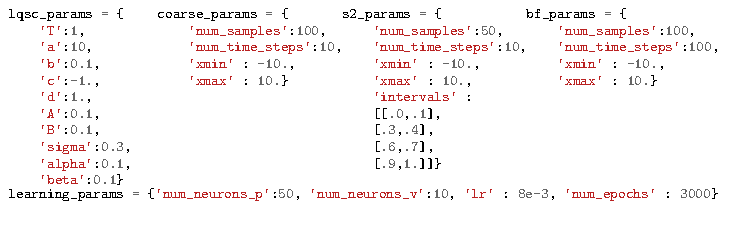
\includegraphics[width=\textwidth]{figures/ms2_params.pdf}
\caption{The choice of parameters for the LQSC problem as well as the the first (coarse) and second step (s2) of multi-scale method and the brute-force (bf) method.}
    \label{params}
\end{figure}

% Figure~\ref{fig:value_comparison_bw_brute_multi} shows the comparison between the approximation of cost, value function, at time $0$, between the $2$-fold multi-scale PGM method and the brute-force PGM for 100 steps. While the brute-force PGM shows slightly less error, it takes $203$ seconds to run with $3,000$ training epochs. The $2$-fold multi-scale  PGM takes $35$ seconds with the same number of epochs, resulting in an approximate $82\%$ reduction in training time.

% \begin{figure}[ht!]
%     \centering
%     \includegraphics[width=0.8\linewidth]{figures/Optimal_soln_LQC.eps}
%     \caption{Comparison of the $2$-fold PGM and the closed-from optimal policy for different values of $x$.}
%     \label{fig:policy_comparison_w_closed}
% \end{figure}

% \begin{figure}[ht!]
%     \centering
%     \includegraphics[width=0.8\linewidth]{figures/Prcnt_er_LQC_a10.eps}
%     \caption{Comparison of the error of value function between $2$-fold PGM and the brute-force PGM for $100$ time steps.}
%     \label{fig:value_comparison_bw_brute_multi}
% \end{figure}
\begin{remark}
    [Choice of parameters]
    We should emphasize that the problems of interest are the ones that a coarse discretization does not provide a relatively accurate solution for the continuous-time problem. The choice of parameters for the linear-quadratic stochastic control problem in our numerical experiment is such that the coarse discretization has a relatively large error and only when we refine the discretization, we obtain an accurate solution. To achieve that, we need functions $f(t)$ and $h(t)$ in \eqref{Riccati} to vary significantly in time. One of the way to achieve this variation is to choose the parameter $A$  relatively large, as we did in our case.
\end{remark}

\begin{figure}[ht!]
    \centering
    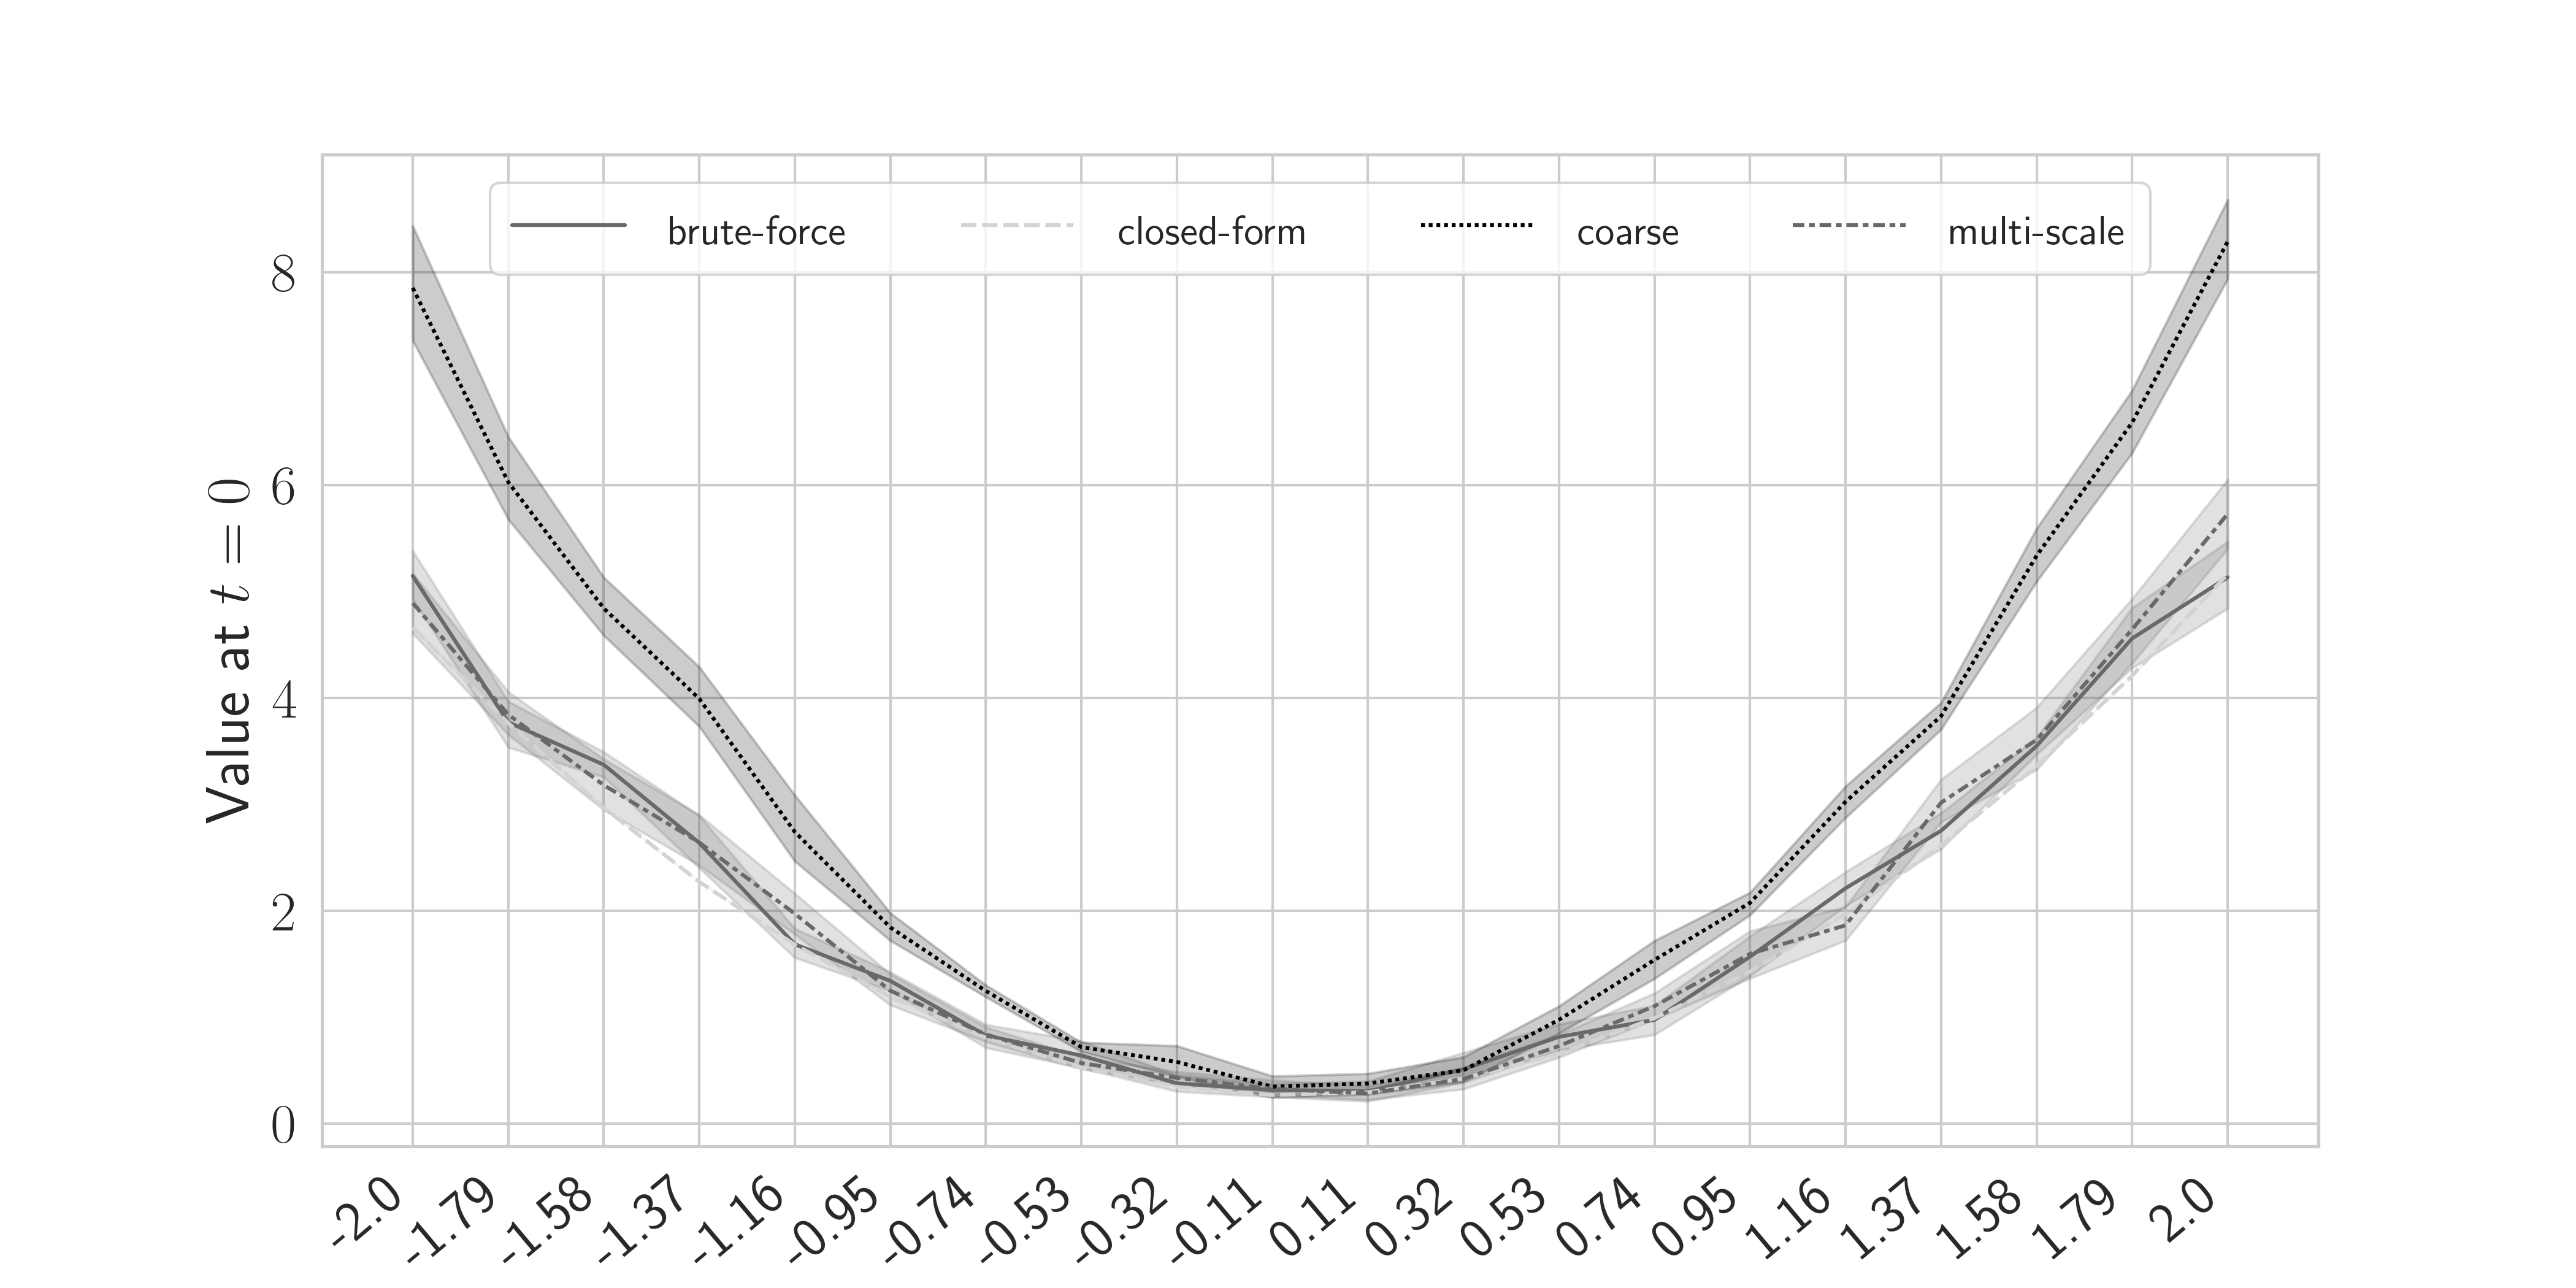
\includegraphics[width=1\linewidth]{figures/bf_100_50_7.png}
    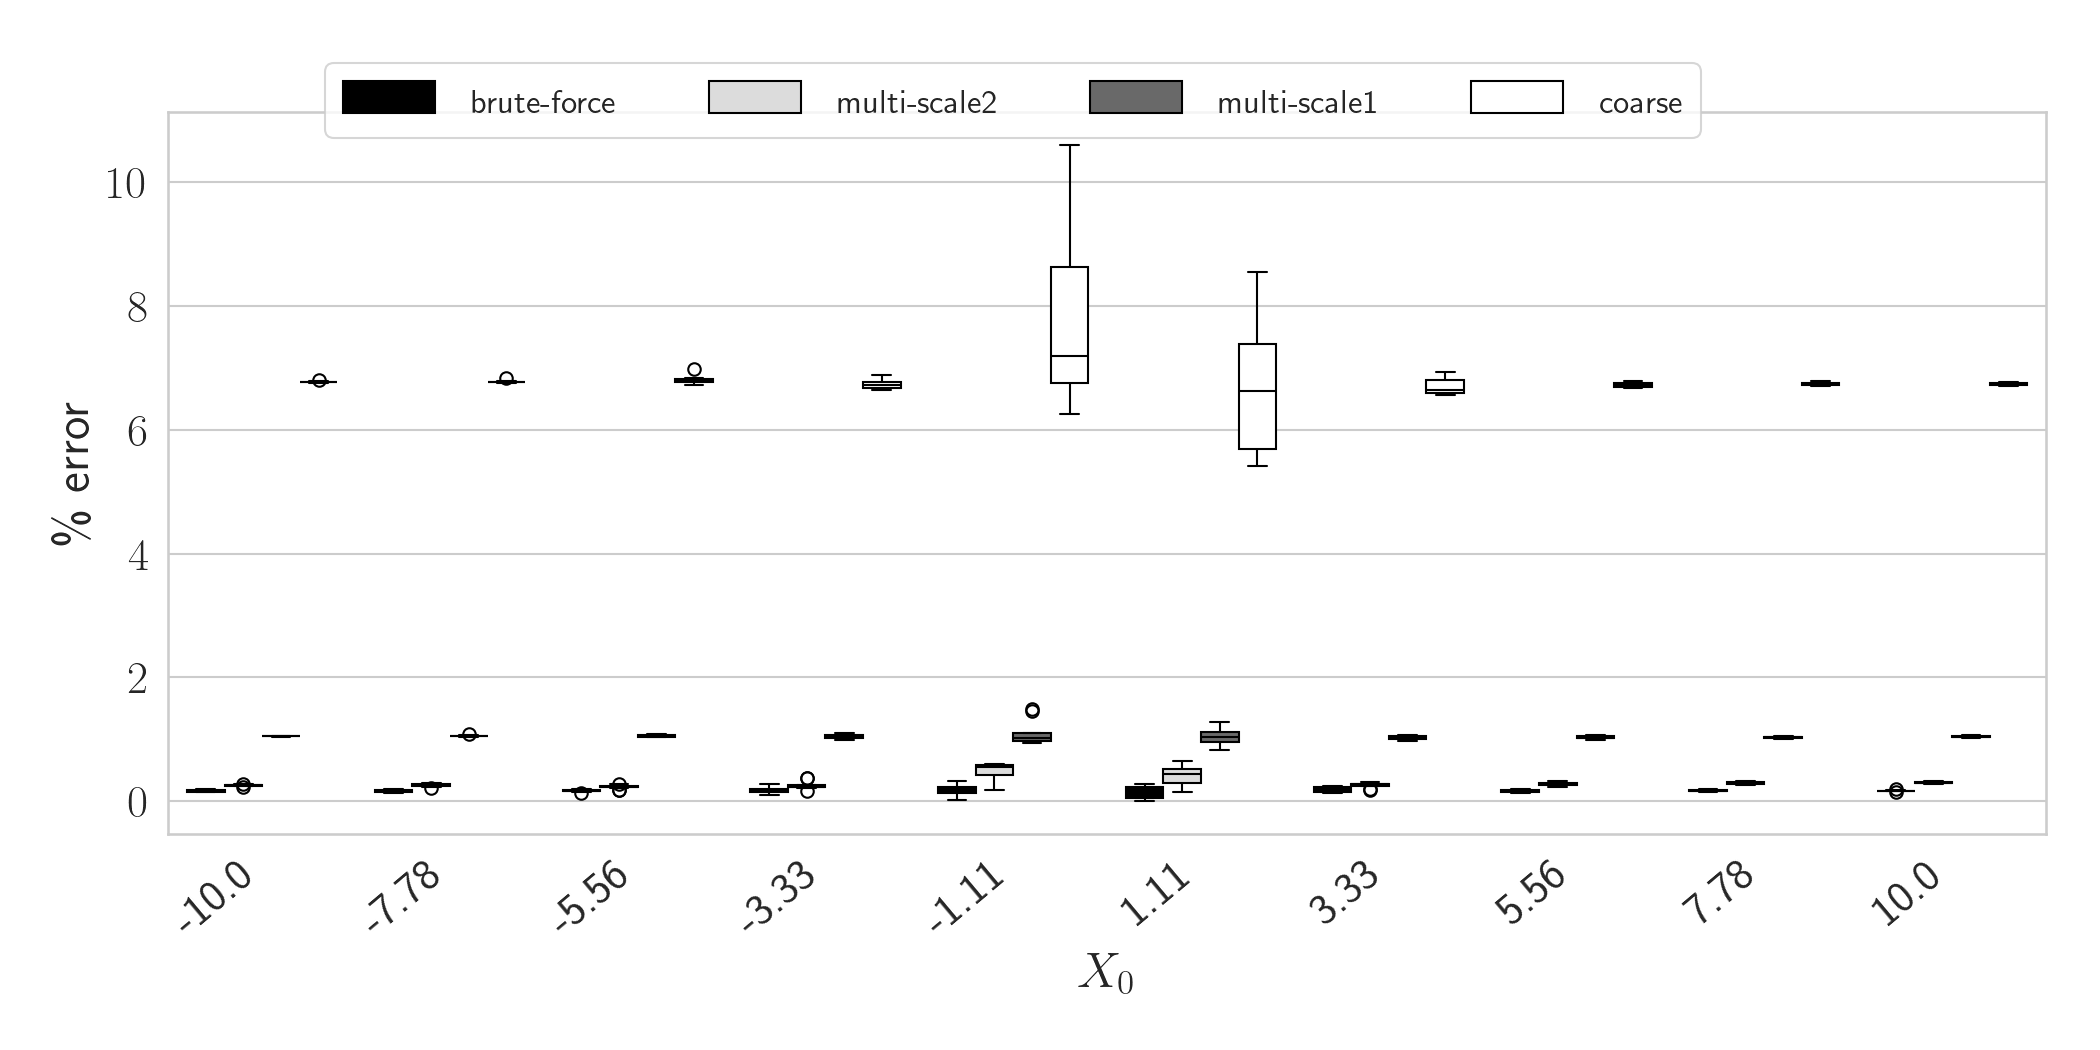
\includegraphics[width=.9\linewidth]{figures/rel_100_50_5_Comparison_bf_ms2_coarse_7.png}
    \caption{Comparison of the cost function between $2$-fold PGM and brute-force PGM with the closed-form solutions in for $100$ time steps in 10 independent runs.}
    \label{fig:value0_comparison_bw_brute_multi}
\end{figure}

\subsection{Three-fold multi-scale experiment}
As seen in Listing~\eqref{params2}, for this experiment, we modify the coefficient $a$ from $10$ to $100$ to create more variation in time variable. We choose $N=5$, $J=100$, $J_1=100$, $J_2=50$, and $J_3=5$. We choose three intervals, $[0.0,0.25]$, $[0.5,0.75]$, and $[1.0,1.25]$ for training in the second step and five intervals, $[0.0, 0.05]$, $[0.3, 0.35]$, $[0.6, 0.65]$, $[0.9, 0.95]$, $[1.2, 1.25]$ for training in the third step. 

\begin{figure}[H]\centering
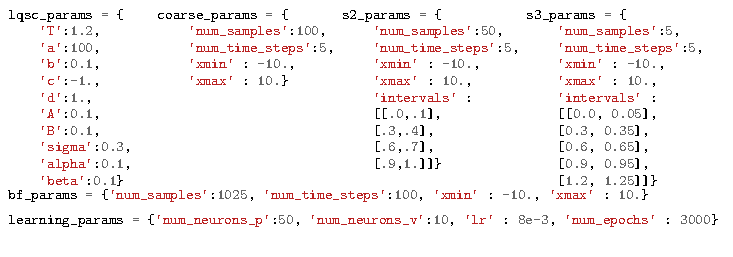
\includegraphics[width=\textwidth]{figures/ms3_params.pdf}
\caption{The choice of parameters for the LQSC problem as well as the the first (coarse) and second and third steps (s2 and s3) of multi-scale method and the brute-force (bf) method.}
    \label{params2}
\end{figure}

The three-fold multi-scale PGM runs in $94$ seconds compare to $160$ seconds for the brute-force PGM.

\begin{figure}[ht!]
    \centering
    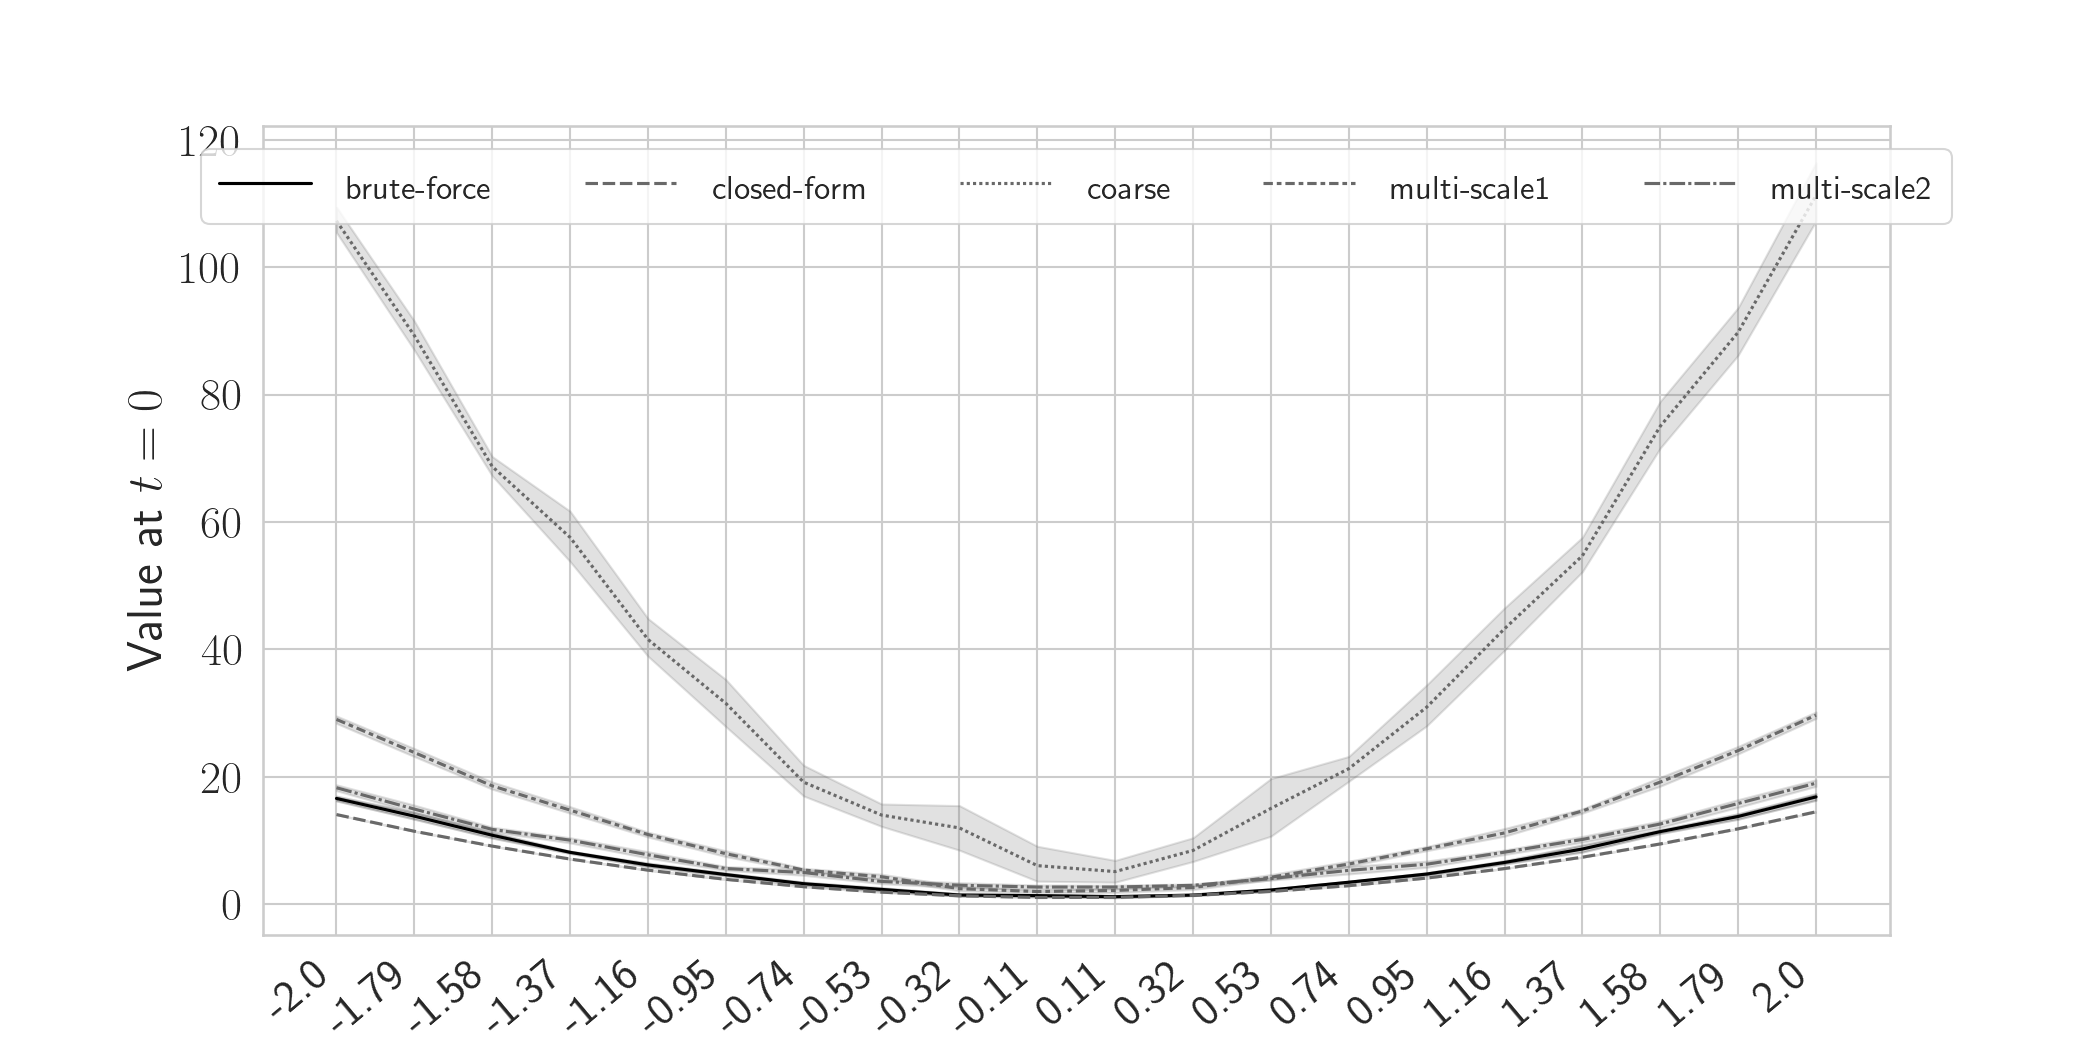
\includegraphics[width=1\linewidth]{figures/bf_100_50_5_8.png}
    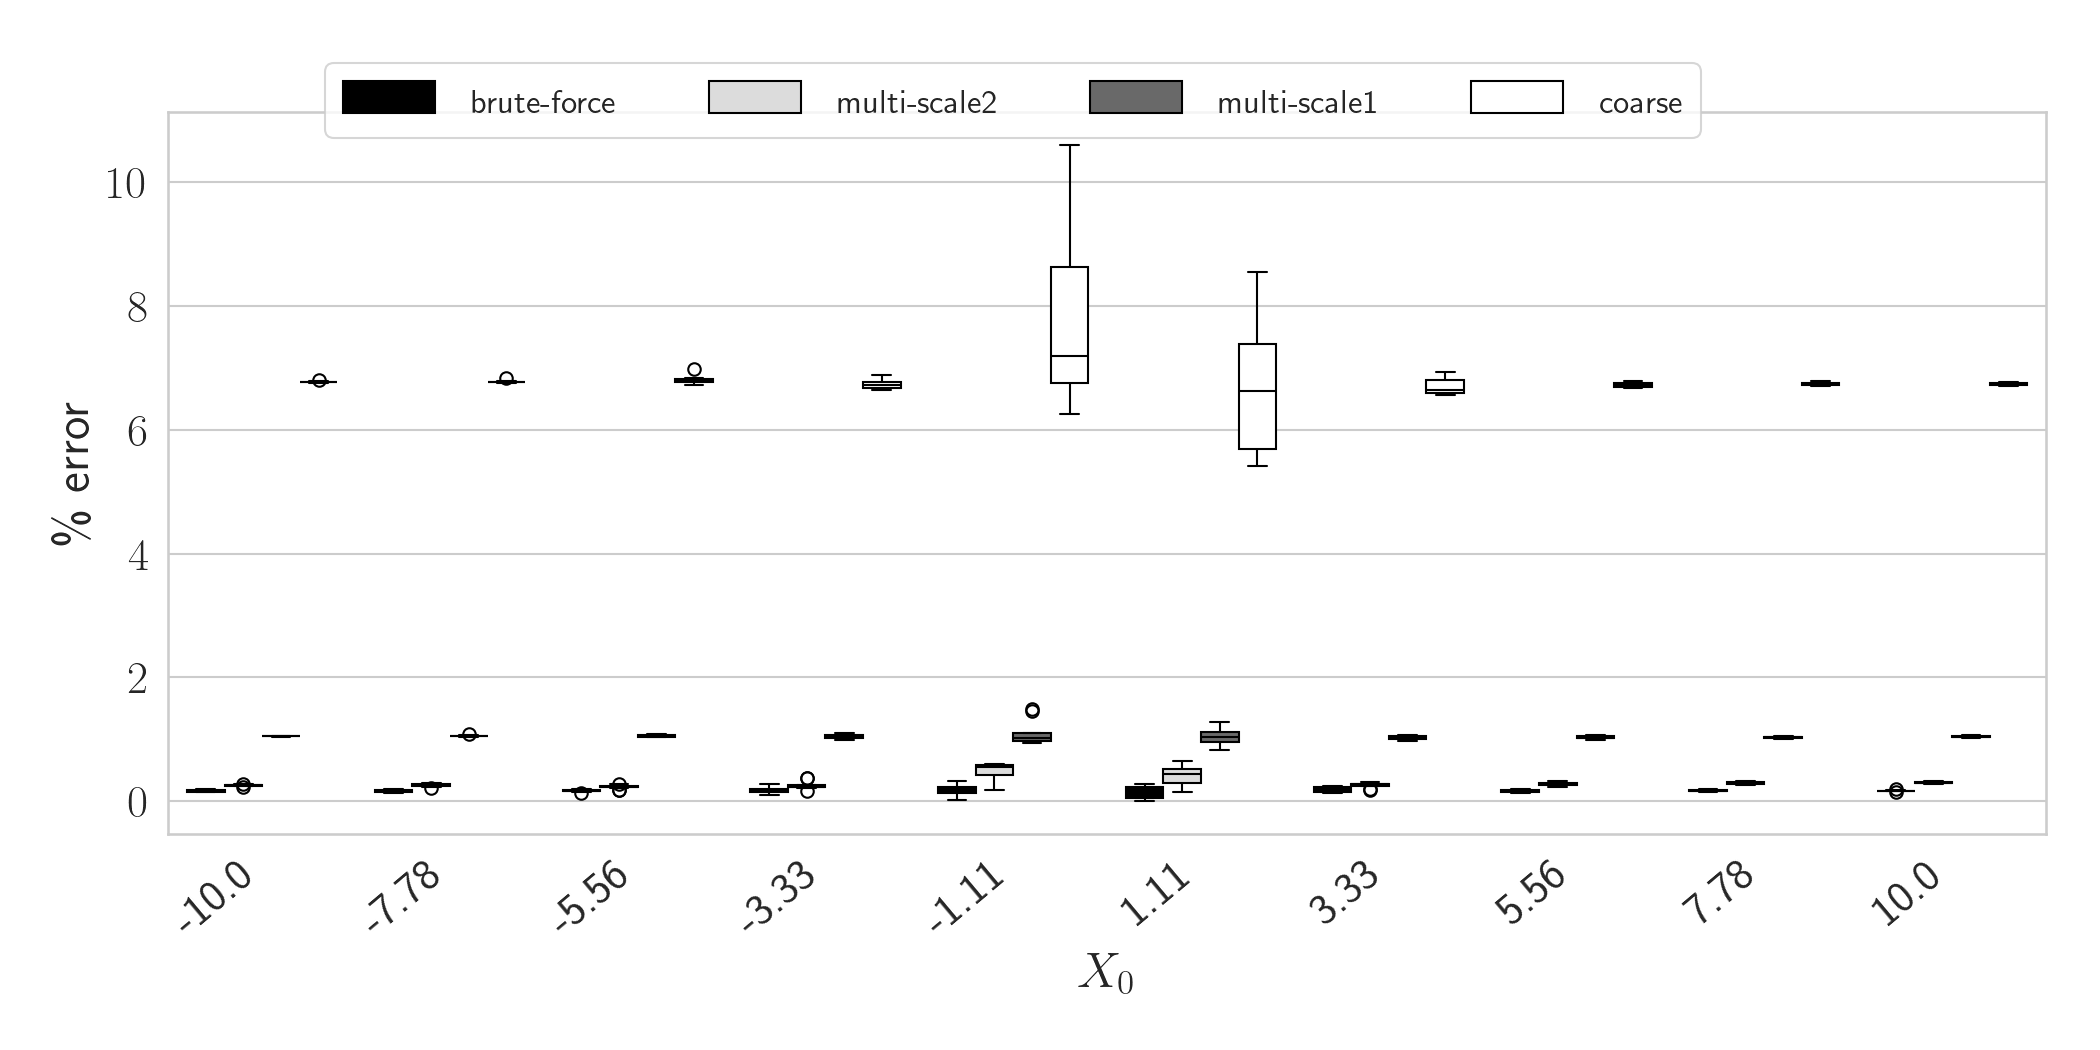
\includegraphics[width=.9\linewidth]{figures/rel_100_50_5_Comparison_bf_ms2_coarse_7.png}
    \caption{Comparison of the cost function between $3$-fold PGM and brute-force PGM with the closed-form solutions in for $125$ time steps in 10 independent runs.}
    \label{fig:value2_comparison_bw_brute_multi}
\end{figure}
%%%%%%%%%%%%%%%%%%%%%%%%%%%%%%%%%%%%%%%%%%%%%%
%%%%%%%%%%%%%%%%%%%%%%%%%%%%%%%%%%%%%%%%%%%%%%
%%%%%%%%%%%%%%%%%%%%%%%%%%%%%%%%%%%%%%%%%%%%%%
\section{Conclusion}
In this paper, we proposed a method, which allows to improve the efficiency of the policy gradient method for optimal control problems via a multi-step/multi-scale implementation. Our method is useful for problems which the coarse discretization does not provide a sufficiently accurate approximation and finer time discretization is required, specifically, if the cost varies significantly in time. We tested our method on a linear-quadratic stochastic control problem, which has a closed-form solution and compared the results of two and three-step implementations. Additionally, we provide a theoretical result on the computational complexity of the algorithm on the number of steps, number of time intervals used in each step, and number of samples in each step. This result also allows to set these parameters to reduce the run-time of the multi-scale policy gradient method by a given factor.


 \appendix
 \section{Proof of Theorem~\ref{thm:strong_error}}
 \label{sec:error}
 In this appendix, we provide a proof of the error bound for approximation of the continuous-time control problem with the discretized version stated in Theorem~\ref{thm:strong_error}. Although it is an standard result, we provide it for the sake of completion. We first assume the following:
 \begin{enumerate}[label=\bfseries A.\arabic*.]
     \item There exists an optimal Markovian control $\pi^*_t= \phi(t,X^*_t)\in\Uppi$ for \eqref{prob:control} such that $\phi(t,x)$ is jointly measurable in $(t,x)$ and $\nicefrac{1}{2}$-Hölder continuous in $t$ and Lipschitz in $x$ uniformly.
     \item $L(t,x,p)$, $\mu(t,x,p)$, $\sigma(t,x,p)$, and $g(x)$ are Lipschitz on $x$ uniform in$(t,\pi)$ and  $L(t,x,p)$ is $\nicefrac{1}{2}$-Hölder continuous in $t$ uniformly in $(x,p)$.
      \item The piecewise constant control $\hat{\pi}^*_t=\phi(t_{i},\hat{X}^*_{t_{i}})$ for $t\in[t_i,t_{i+1}]$ belongs to $\Uppi$ and constitute an admissible control for \eqref{prob:control_discretized}.
      % \item Not any positive integer $n$, there exists an optimal Markovian control $\pi^{*n}_{t_i}= \phi^n({t_i},\hat{X}^{*n}_t)\in\Uppi$ for \eqref{prob:control} such that $\phi^n(t,x)$ is  Lipschitz in $x$ and the Lipschitz constant can be chosen independent of $n$.
     \item For any positive integer $n$, there exists a optimal policy $\pi^{*n}_{t_i}=\phi^n(t_i,\hat{X}^*_{t_i})\in\Uppi$ for the discretized problem \eqref{prob:control_discretized}.
 \end{enumerate}
 Assumption \textbf{A.1} implies that 
 \begin{equation}
    V(t,x)=\mathbb{E}\left[\int_t^TL(s,X^*_s,\phi(s,X^*_s))ds + g(X_T^*)\bigg| X_t^*=x\right] 
\end{equation}
where 
\begin{equation}\label{eqn:X^*}
    dX^*_t =\mu(t,X_t^*,\phi(t,X^*_t))dt+\sigma(t,X^*_t,\phi(t,X^*_t))dW_t
\end{equation} 
and let $\hat{X}^*_t$ be the Euler discretization of the SDE \eqref{eqn:X^*}. 
Further define  
\begin{equation}
\begin{split}
    \hat{U}^*(t_{i},x)&:=\mathbb{E}\left[\sum_{\hat{i}\in[n-i]}L(t_{i+\hat{i}},\hat{X}^*_{t_{i+\hat{i}}},\hat{\pi}^*_{t_{i+\hat{i}}})\delta + g(\hat{X}_T^{*})\bigg|\hat{X}^{*}_{t_i}=x\right]\\
    {U}^*(t,x)&:=\mathbb{E}\left[\int_t^T L(s,\hat{X}^*_{s},\hat{\pi}^*_s)ds + g(\hat{X}_T^{*})\bigg|\hat{X}^{*}_{t}=x\right]
\end{split}
\end{equation}
$\hat{\pi}^*_t=\phi(t_{i},\hat{X}^*_{t_{i}})$ for $t\in[t_i,t_{i+1})$.
Note that, by Assumption \textbf{A.3}, 
\begin{equation}
    \hat{U}^*(t_{i},x) = \mathcal{J}^n(\hat{\pi}^*)\ge \hat{V}(t_i,x)
\end{equation}
where  that $\hat{V}$ is the value function of the discretized problem defined in \eqref{defn:value_discrete}.
Thus, 
\begin{equation}
    \begin{split}
        \hat{V}(t_{i},x)-{V}(t_{i},x)\le  & \hat{U}^*(t_{i},x)-{V}(t_{i},x)\\
        \le & \hat{U}^*(t_{i},x)-
        U^*(t_{i},x)+{U}^*(t_{i},x)-{V}(t_{i},x)
    \end{split}
\end{equation}
By Assumption \textbf{A.2},  $\nicefrac{1}{2}$-Hölder continuous  of $L$ in $t$ and Lipschitz continuity of $L$ in $x$, we have 
\begin{equation}
\begin{split}
    \bigg|\int_{t_{j}}^{t_{j+1}} &\!\!\!\!\!\!\! L(s,\hat{X}^*_{s},\hat{\pi}^*_{s})ds-L(t_{j},\hat{X}^*_{t_{j}},\hat{\pi}^*_{t_j})\delta\bigg|\le \int_{t_{j}}^{t_{j+1}} \!\!\!\!\!\!\!\big|L(s,\hat{X}^*_{s},\hat{\pi}^*_{s})-L(t_{j},\hat{X}^*_{t_{j}},\hat{\pi}^*_{t_j})\big|ds\\
    = &\int_{t_{j}}^{t_{j+1}} \!\!\!\!\!\!\! \big|L(s,\hat{X}^*_{s},\hat{\pi}^*_{t_j})-L(t_{j},\hat{X}^*_{t_{j}},\hat{\pi}^*_{t_j})\big|ds \le  C \int_{t_{j}}^{t_{j+1}}\!\!\!\!\!\!\! (\sqrt{s-t_j}+|\hat{X}^*_{s}-\hat{X}^*_{t_{j}}|)ds
\end{split}
\end{equation}
Therefore, 
\begin{equation}\label{eqn:hatU-U-int}
    |\hat{U}^*(t_{i},x)-{U}^*(t_{i},x)|\le C\sum_{i\le j\le N-1} \int_{t_{j}}^{t_{j+1}}\!\!\!\!\!\!\! (\sqrt{s-t_j}+\mathbb{E}[|\hat{X}^*_{s}-\hat{X}^*_{t_{j}}|])ds
\end{equation}
Since $\mathbb{E}[|\hat{X}^*_{s}-\hat{X}^*_{t_{j}}|]\le C\sqrt{s-t_j}$, after integrating the right-hand side of \eqref{eqn:hatU-U-int}, we obtain
\begin{equation}\label{eqn:hatU-U}
    |{U}^*(t_{i},x)-\hat{U}^*(t_{i},x)|\le C\sqrt{\delta}.
\end{equation}
One the other hand, by Assumption \textbf{A1}, for $s\in[t_{i},t_{i+1}]$, we have
\begin{equation}\label{phi-phi}
    |\phi(t_i,\hat{X}_{t_i}^{*})-\phi(s,{X}_{s}^{*})|\le C(\sqrt{s-t_j}+|\hat{X}^*_{s}-{X}^*_{t_i}|)
\end{equation}
Therefore, we can use \eqref{phi-phi} and Lipschitz assumption on $L$ and $g$ to write
\begin{equation}\label{eqn:U*-V}
    \begin{split}
        0&\le {U}^*(t_{i},x) -V(t_{i},x)\\
        &\le \mathbb{E}\bigg[ \int_t^T \!\!\!\!\!\big(L(s,\hat{X}^*_{s},\hat{\pi}^*_s)-L(s,{X}^*_{s},{\pi}^*_s)\big)ds + g(\hat{X}_T^{*})- g({X}_T^{*})  \bigg] \\
        &\le C\mathbb{E}\bigg[ \int_t^T \big(\sqrt{s-t_j}+|\hat{X}^*_{s}-{X}^*_{t_i}|+|\hat{X}^*_{s}-{X}^*_{s}|\big)ds 
        + |\hat{X}_T^{*} - {X}_T^{*}|  \bigg]\\
        &\le C \big(\sqrt{s-t_j}+\sup_{s\in[t_i,T]}\mathbb{E}[|X^*_{s}-\hat{X}^*_{s}|]\big)\le C\sqrt{\delta}
    \end{split}
\end{equation}
In the above, the last inequality follows from $\sup_{t\in[0,T]}\mathbb{E}[|\hat{X}^*_{t}-{X}^*_{t}|]\le C\sqrt{\delta}$ which comes from \citet[Theorem~9.6.2]{KP13} and the second to last inequality follows from $\mathbb{E}[|\hat{X}^*_{s}-\hat{X}^*_{t_{j}}|]\le C\sqrt{s-t_j}$. 
Here, $C$ only depends on the Lipschitz constants and $\nicefrac{1}{2}$-Hölder constant from Assumption \textbf{A.2}. By \eqref{eqn:hatU-U} and \eqref{eqn:U*-V}, we obtain
\begin{equation}
    \begin{split}
        \sup_{x, i\in[N]}\hat{V}(t_{i},x)-{V}(t_{i},x)\le  \sup_{x, i\in[N]} \big(&|U^*(t_{i},x)-\hat{U}^*(t_{i},x)|\\
        &+|\hat{U}^*(t_{i},x)-\hat{V}(t_{i},x)|\big) \le C\sqrt{\delta}
    \end{split}
\end{equation}
To show that 
Similarly, one can show that $\sup_{x, i\in[N]}\hat{V}(t_{i},x)-{V}(t_{i},x)\le C\sqrt{\delta}$, we consider a continuous-time strategy constructed on the discrete-time strategy provided by Assumption~\textbf{A.4} defined by 
$\pi_t:=\phi^n(t_i,X^{*n}_{t_i})$ for $t\in[t_i,t_{i+1})$, where $X^{*n}$ is the optimal trajectory for the discrete problem \eqref{prob:control_discretized}. Therefore, we have 
\begin{equation}
    \hat{V}(t_i,x)=\mathbb{E}\left[\sum_{\hat{i}\in[n-i]}L(t_{i+\hat{i}},\hat{X}^{*n}_{t_{i+\hat{i}}},{\pi}_{t_{i+\hat{i}}})\delta + g(\hat{X}_T^{*})\bigg|\hat{X}^{*n}_{t_i}=x\right]
\end{equation}
Define
\begin{equation}
\begin{split}
    {U}(t_i,x)&:=\mathbb{E}\left[\int_{t_i}^T L(s,{X}^{\pi}_{s},{\pi}_s)ds + g({X}^{\pi}_T)\bigg|{X}_{t_i}=x\right]
\end{split}
\end{equation}
Note that ${\pi}$ is a delayed control for the continuous-time problem, which depends only on the state variable at  the last discrete time step and agrees with the discrete-time optimal control on the time grid. 
Therefore, we have  ${\pi}_s={\pi}_{t_i}$ on $s\in[t_i,t_{i+1})$ and ${U}(t,x) = \mathfrak{J}({\pi})\ge V(t,x)$
\begin{equation}
\begin{split}
    &\bigg|\int_{t_{j}}^{t_{j+1}} \!\!\!\!\!\!\! L(s,{X}^{\pi}_{s},{\pi}_{s})ds-L(t_{j},\hat{X}^{*n}_{t_{j}},{\pi}_{t_j})\delta\bigg|\le \int_{t_{j}}^{t_{j+1}} \!\!\!\!\!\!\!\big|L(s,{X}^\pi_{s},{\pi}_{s})-L(t_{j},\hat{X}^{*n}_{t_{j}},{\pi}_{t_j})\big|ds\\
    = &\int_{t_{j}}^{t_{j+1}} \!\!\!\!\Big(\big|L(s,\hat{X}^{*n}_{t_{j}},{\pi}_{t_i})-L(t_{j},\hat{X}^{*n}_{t_{j}},{\pi}_{t_j})\big|+\big|L(s,{X}^\pi_{t_{j}},{\pi}_{t_i})-L(s,\hat{X}^{*n}_{t_{j}},{\pi}_{t_j})\big|\Big)ds
\end{split}
\end{equation}
By Hölder continuity assumption, we have
\begin{equation}\label{Ls-Lt_j}
    |L(s,\hat{X}^{*n}_{t_{j}},{\pi}_{t_i})-L(t_{j},\hat{X}^{*n}_{t_{j}},{\pi}_{t_j})\big|\le C \sqrt{s-t_j}
\end{equation}
Furthermore, we have 
\begin{equation}\label{X_pi-X*}
\begin{split}
     \big|L(s,{X}^\pi_{s},{\pi}_{t_i})-L(s,\hat{X}^{*n}_{t_{j}},{\pi}_{t_j})\big|\le C (|{X}^\pi_{s}-{X}^{\pi}_{t_{j}}|+ |{X}^\pi_{t_i}-\hat{X}^{*n}_{t_{j}}|)
\end{split}
\end{equation}
Note that $\mathbb{E}[|{X}^\pi_{s}-{X}^{\pi}_{t_{j}}|]\le \sqrt{s-t_j}$. 
Because the difference between the drift and diffusion coefficient of ${X}^\pi$ and $\hat{X}^{*n}$ is bounded by $C\sqrt{\delta}$, we can show that $\mathbb{E}[|{X}^\pi_{t_j}-\hat{X}^{*n}_{t_{j}}|]\le C\sqrt{\delta}$.
Estimates \eqref{Ls-Lt_j} and \eqref{X_pi-X*} imply that
\begin{equation}\label{eqn:tildeU-U-int}
    |\hat{V}(t_{i},x)-{U}(t_{i},x)|\le C\sum_{i\le j\le N-1} \int_{t_{j}}^{t_{j+1}}\!\!\!\!\!\!\! \sqrt{s-t_j}ds\le C\sqrt{\delta}
\end{equation}
and we have 
\begin{equation}
    \begin{split}
        \sup_{x, i\in[N]}{V}(t_{i},x)-\hat{V}(t_{i},x)\le  \sup_{x, i\in[N]} \big(&|\tilde U(t_{i},x)-\hat{V}(t_{i},x)|\le C\sqrt{\delta}
    \end{split}
\end{equation}
% On the other hand, 

% by \citet[Theorem~9.6.2]{KP13} and Assumption \textbf{A.2}, we have $\sup_{t\in[0,T]}\mathbb{E}[|{X}^{\pi}_{t}-{X}^{*n}_{t}|\le C\sqrt{\delta}$. 
% $\mathbb{E}[|{X}^\pi_{s}-\hat{X}^\pi_{t_{j}}|]\le C\sqrt{s-t_j}$

% In this section, we apply the proposed method on problems rising in optimal execution under different price impact. Some of such problems have closed-from solutions, for example \citet{AFS08} provide a closed-form solution to the \citet{OW13} model. Extensions of \citet{OW13}, including \citet{FSU14} and \citet{FSU19} provide a characterization for the optimal execution strategy, which can lead to a closed-form solution. The drawback of the optimal execution problem is that the quadratic term in the running loss function vanishes as we pass to a continuous-time limit.
% In the spirit of \citet{AKU24}, which shows an optimal execution problem can be reduced to a linear-quadratic optimal control problem, we apply out method on a linear-quadratic optimal control problem, which can easily be compared with the continuous-time closed-from solution.
% \begin{figure}
%     \centering
% % This file was created with tikzplotlib v0.10.1.
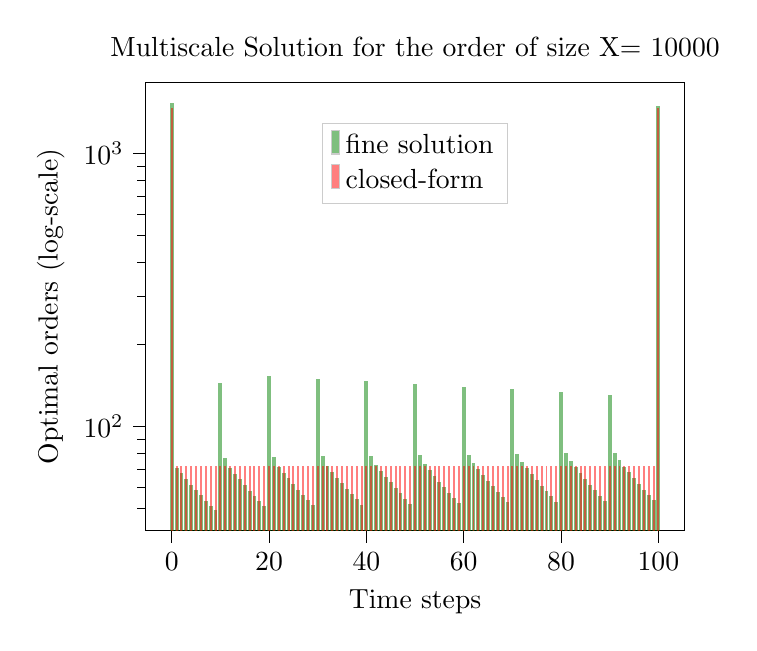
\begin{tikzpicture}

\definecolor{darkgray176}{RGB}{176,176,176}
\definecolor{green}{RGB}{0,128,0}
\definecolor{lightgray204}{RGB}{204,204,204}

\begin{axis}[
legend cell align={left},
legend style={
  fill opacity=0.5,
  draw opacity=1,
  text opacity=1,
  at={(0.5,0.91)},
  anchor=north,
  draw=lightgray204,
  legend entries={fine solution,
                closed-form},
    },
   legend image code/.code={%
    \draw[#1] (0cm,-0.1cm) rectangle (0.1cm,0.2cm);
    }, 
tick align=outside,
tick pos=left,
title={Multiscale Solution for the order of size X= 10000},
x grid style={darkgray176},
xlabel={Time steps},
xmin=-5.44, xmax=105.44,
xtick style={color=black},
y grid style={darkgray176},
ylabel={Optimal orders},
log basis y={10},
x grid style={darkgray176},
xlabel={Time steps},
xmin=-5.44, xmax=105.44,
ylabel={Optimal orders (log-scale)},
ymin=41.5197294792376, ymax=1820.03505338654,
ymode=log,
ytick style={color=black}
]
\addlegendimage{only marks, fill=green}
\draw[draw=none,fill=green,fill opacity=0.5] (axis cs:-0.4,0) rectangle (axis cs:0.4,1532.67944335938);
\draw[draw=none,fill=green,fill opacity=0.5] (axis cs:0.6,0) rectangle (axis cs:1.4,70.8013763427734);
\draw[draw=none,fill=green,fill opacity=0.5] (axis cs:1.6,0) rectangle (axis cs:2.4,67.3683166503906);
\draw[draw=none,fill=green,fill opacity=0.5] (axis cs:2.6,0) rectangle (axis cs:3.4,64.1892547607422);
\draw[draw=none,fill=green,fill opacity=0.5] (axis cs:3.6,0) rectangle (axis cs:4.4,61.2411003112793);
\draw[draw=none,fill=green,fill opacity=0.5] (axis cs:4.6,0) rectangle (axis cs:5.4,58.5031318664551);
\draw[draw=none,fill=green,fill opacity=0.5] (axis cs:5.6,0) rectangle (axis cs:6.4,55.9566230773926);
\draw[draw=none,fill=green,fill opacity=0.5] (axis cs:6.6,0) rectangle (axis cs:7.4,53.584587097168);
\draw[draw=none,fill=green,fill opacity=0.5] (axis cs:7.6,0) rectangle (axis cs:8.4,51.3716735839844);
\draw[draw=none,fill=green,fill opacity=0.5] (axis cs:8.6,0) rectangle (axis cs:9.4,49.3040885925293);
\draw[draw=none,fill=green,fill opacity=0.5] (axis cs:9.6,0) rectangle (axis cs:10.4,144.048263549805);
\draw[draw=none,fill=green,fill opacity=0.5] (axis cs:10.6,0) rectangle (axis cs:11.4,76.6953277587891);
\draw[draw=none,fill=green,fill opacity=0.5] (axis cs:11.6,0) rectangle (axis cs:12.4,70.745002746582);
\draw[draw=none,fill=green,fill opacity=0.5] (axis cs:12.6,0) rectangle (axis cs:13.4,67.2651062011719);
\draw[draw=none,fill=green,fill opacity=0.5] (axis cs:13.6,0) rectangle (axis cs:14.4,64.0450897216797);
\draw[draw=none,fill=green,fill opacity=0.5] (axis cs:14.6,0) rectangle (axis cs:15.4,61.0613594055176);
\draw[draw=none,fill=green,fill opacity=0.5] (axis cs:15.6,0) rectangle (axis cs:16.4,58.2926216125488);
\draw[draw=none,fill=green,fill opacity=0.5] (axis cs:16.6,0) rectangle (axis cs:17.4,55.7195434570312);
\draw[draw=none,fill=green,fill opacity=0.5] (axis cs:17.6,0) rectangle (axis cs:18.4,53.3247756958008);
\draw[draw=none,fill=green,fill opacity=0.5] (axis cs:18.6,0) rectangle (axis cs:19.4,51.0925598144531);
\draw[draw=none,fill=green,fill opacity=0.5] (axis cs:19.6,0) rectangle (axis cs:20.4,153.40788269043);
\draw[draw=none,fill=green,fill opacity=0.5] (axis cs:20.6,0) rectangle (axis cs:21.4,77.2673187255859);
\draw[draw=none,fill=green,fill opacity=0.5] (axis cs:21.6,0) rectangle (axis cs:22.4,71.3731384277344);
\draw[draw=none,fill=green,fill opacity=0.5] (axis cs:22.6,0) rectangle (axis cs:23.4,67.8467788696289);
\draw[draw=none,fill=green,fill opacity=0.5] (axis cs:23.6,0) rectangle (axis cs:24.4,64.584587097168);
\draw[draw=none,fill=green,fill opacity=0.5] (axis cs:24.6,0) rectangle (axis cs:25.4,61.5623817443848);
\draw[draw=none,fill=green,fill opacity=0.5] (axis cs:25.6,0) rectangle (axis cs:26.4,58.758617401123);
\draw[draw=none,fill=green,fill opacity=0.5] (axis cs:26.6,0) rectangle (axis cs:27.4,56.1536254882812);
\draw[draw=none,fill=green,fill opacity=0.5] (axis cs:27.6,0) rectangle (axis cs:28.4,53.7297897338867);
\draw[draw=none,fill=green,fill opacity=0.5] (axis cs:28.6,0) rectangle (axis cs:29.4,51.4709968566895);
\draw[draw=none,fill=green,fill opacity=0.5] (axis cs:29.6,0) rectangle (axis cs:30.4,149.965942382812);
\draw[draw=none,fill=green,fill opacity=0.5] (axis cs:30.6,0) rectangle (axis cs:31.4,77.7061462402344);
\draw[draw=none,fill=green,fill opacity=0.5] (axis cs:31.6,0) rectangle (axis cs:32.4,71.9484939575195);
\draw[draw=none,fill=green,fill opacity=0.5] (axis cs:32.6,0) rectangle (axis cs:33.4,68.3795013427734);
\draw[draw=none,fill=green,fill opacity=0.5] (axis cs:33.6,0) rectangle (axis cs:34.4,65.0784378051758);
\draw[draw=none,fill=green,fill opacity=0.5] (axis cs:34.6,0) rectangle (axis cs:35.4,62.0209503173828);
\draw[draw=none,fill=green,fill opacity=0.5] (axis cs:35.6,0) rectangle (axis cs:36.4,59.1850967407227);
\draw[draw=none,fill=green,fill opacity=0.5] (axis cs:36.6,0) rectangle (axis cs:37.4,56.5508003234863);
\draw[draw=none,fill=green,fill opacity=0.5] (axis cs:37.6,0) rectangle (axis cs:38.4,54.1002159118652);
\draw[draw=none,fill=green,fill opacity=0.5] (axis cs:38.6,0) rectangle (axis cs:39.4,51.817008972168);
\draw[draw=none,fill=green,fill opacity=0.5] (axis cs:39.6,0) rectangle (axis cs:40.4,146.504699707031);
\draw[draw=none,fill=green,fill opacity=0.5] (axis cs:40.6,0) rectangle (axis cs:41.4,78.1253433227539);
\draw[draw=none,fill=green,fill opacity=0.5] (axis cs:41.6,0) rectangle (axis cs:42.4,72.5057830810547);
\draw[draw=none,fill=green,fill opacity=0.5] (axis cs:42.6,0) rectangle (axis cs:43.4,68.8950347900391);
\draw[draw=none,fill=green,fill opacity=0.5] (axis cs:43.6,0) rectangle (axis cs:44.4,65.5559844970703);
\draw[draw=none,fill=green,fill opacity=0.5] (axis cs:44.6,0) rectangle (axis cs:45.4,62.463996887207);
\draw[draw=none,fill=green,fill opacity=0.5] (axis cs:45.6,0) rectangle (axis cs:46.4,59.5966148376465);
\draw[draw=none,fill=green,fill opacity=0.5] (axis cs:46.6,0) rectangle (axis cs:47.4,56.9337387084961);
\draw[draw=none,fill=green,fill opacity=0.5] (axis cs:47.6,0) rectangle (axis cs:48.4,54.45703125);
\draw[draw=none,fill=green,fill opacity=0.5] (axis cs:48.6,0) rectangle (axis cs:49.4,52.1500129699707);
\draw[draw=none,fill=green,fill opacity=0.5] (axis cs:49.6,0) rectangle (axis cs:50.4,143.147674560547);
\draw[draw=none,fill=green,fill opacity=0.5] (axis cs:50.6,0) rectangle (axis cs:51.4,78.5334167480469);
\draw[draw=none,fill=green,fill opacity=0.5] (axis cs:51.6,0) rectangle (axis cs:52.4,73.0522766113281);
\draw[draw=none,fill=green,fill opacity=0.5] (axis cs:52.6,0) rectangle (axis cs:53.4,69.4002456665039);
\draw[draw=none,fill=green,fill opacity=0.5] (axis cs:53.6,0) rectangle (axis cs:54.4,66.0237579345703);
\draw[draw=none,fill=green,fill opacity=0.5] (axis cs:54.6,0) rectangle (axis cs:55.4,62.897632598877);
\draw[draw=none,fill=green,fill opacity=0.5] (axis cs:55.6,0) rectangle (axis cs:56.4,59.9992027282715);
\draw[draw=none,fill=green,fill opacity=0.5] (axis cs:56.6,0) rectangle (axis cs:57.4,57.3081245422363);
\draw[draw=none,fill=green,fill opacity=0.5] (axis cs:57.6,0) rectangle (axis cs:58.4,54.8056030273438);
\draw[draw=none,fill=green,fill opacity=0.5] (axis cs:58.6,0) rectangle (axis cs:59.4,52.4751472473145);
\draw[draw=none,fill=green,fill opacity=0.5] (axis cs:59.6,0) rectangle (axis cs:60.4,139.887985229492);
\draw[draw=none,fill=green,fill opacity=0.5] (axis cs:60.6,0) rectangle (axis cs:61.4,78.9367752075195);
\draw[draw=none,fill=green,fill opacity=0.5] (axis cs:61.6,0) rectangle (axis cs:62.4,73.5937881469727);
\draw[draw=none,fill=green,fill opacity=0.5] (axis cs:62.6,0) rectangle (axis cs:63.4,69.9007568359375);
\draw[draw=none,fill=green,fill opacity=0.5] (axis cs:63.6,0) rectangle (axis cs:64.4,66.4869842529297);
\draw[draw=none,fill=green,fill opacity=0.5] (axis cs:64.6,0) rectangle (axis cs:65.4,63.3269882202148);
\draw[draw=none,fill=green,fill opacity=0.5] (axis cs:65.6,0) rectangle (axis cs:66.4,60.3977241516113);
\draw[draw=none,fill=green,fill opacity=0.5] (axis cs:66.6,0) rectangle (axis cs:67.4,57.6785354614258);
\draw[draw=none,fill=green,fill opacity=0.5] (axis cs:67.6,0) rectangle (axis cs:68.4,55.1504745483398);
\draw[draw=none,fill=green,fill opacity=0.5] (axis cs:68.6,0) rectangle (axis cs:69.4,52.7966957092285);
\draw[draw=none,fill=green,fill opacity=0.5] (axis cs:69.6,0) rectangle (axis cs:70.4,136.715515136719);
\draw[draw=none,fill=green,fill opacity=0.5] (axis cs:70.6,0) rectangle (axis cs:71.4,79.3403015136719);
\draw[draw=none,fill=green,fill opacity=0.5] (axis cs:71.6,0) rectangle (axis cs:72.4,74.1349792480469);
\draw[draw=none,fill=green,fill opacity=0.5] (axis cs:72.6,0) rectangle (axis cs:73.4,70.4009323120117);
\draw[draw=none,fill=green,fill opacity=0.5] (axis cs:73.6,0) rectangle (axis cs:74.4,66.9499053955078);
\draw[draw=none,fill=green,fill opacity=0.5] (axis cs:74.6,0) rectangle (axis cs:75.4,63.755989074707);
\draw[draw=none,fill=green,fill opacity=0.5] (axis cs:75.6,0) rectangle (axis cs:76.4,60.7959861755371);
\draw[draw=none,fill=green,fill opacity=0.5] (axis cs:76.6,0) rectangle (axis cs:77.4,58.0486640930176);
\draw[draw=none,fill=green,fill opacity=0.5] (axis cs:77.6,0) rectangle (axis cs:78.4,55.4950637817383);
\draw[draw=none,fill=green,fill opacity=0.5] (axis cs:78.6,0) rectangle (axis cs:79.4,53.1178894042969);
\draw[draw=none,fill=green,fill opacity=0.5] (axis cs:79.6,0) rectangle (axis cs:80.4,133.622543334961);
\draw[draw=none,fill=green,fill opacity=0.5] (axis cs:80.6,0) rectangle (axis cs:81.4,79.7480621337891);
\draw[draw=none,fill=green,fill opacity=0.5] (axis cs:81.6,0) rectangle (axis cs:82.4,74.6796646118164);
\draw[draw=none,fill=green,fill opacity=0.5] (axis cs:82.6,0) rectangle (axis cs:83.4,70.9044647216797);
\draw[draw=none,fill=green,fill opacity=0.5] (axis cs:83.6,0) rectangle (axis cs:84.4,67.4159393310547);
\draw[draw=none,fill=green,fill opacity=0.5] (axis cs:84.6,0) rectangle (axis cs:85.4,64.1879959106445);
\draw[draw=none,fill=green,fill opacity=0.5] (axis cs:85.6,0) rectangle (axis cs:86.4,61.197021484375);
\draw[draw=none,fill=green,fill opacity=0.5] (axis cs:86.6,0) rectangle (axis cs:87.4,58.4215354919434);
\draw[draw=none,fill=green,fill opacity=0.5] (axis cs:87.6,0) rectangle (axis cs:88.4,55.8421936035156);
\draw[draw=none,fill=green,fill opacity=0.5] (axis cs:88.6,0) rectangle (axis cs:89.4,53.4416275024414);
\draw[draw=none,fill=green,fill opacity=0.5] (axis cs:89.6,0) rectangle (axis cs:90.4,130.549713134766);
\draw[draw=none,fill=green,fill opacity=0.5] (axis cs:90.6,0) rectangle (axis cs:91.4,80.1599578857422);
\draw[draw=none,fill=green,fill opacity=0.5] (axis cs:91.6,0) rectangle (axis cs:92.4,75.2281875610352);
\draw[draw=none,fill=green,fill opacity=0.5] (axis cs:92.6,0) rectangle (axis cs:93.4,71.4115524291992);
\draw[draw=none,fill=green,fill opacity=0.5] (axis cs:93.6,0) rectangle (axis cs:94.4,67.885498046875);
\draw[draw=none,fill=green,fill opacity=0.5] (axis cs:94.6,0) rectangle (axis cs:95.4,64.6233291625977);
\draw[draw=none,fill=green,fill opacity=0.5] (axis cs:95.6,0) rectangle (axis cs:96.4,61.6012229919434);
\draw[draw=none,fill=green,fill opacity=0.5] (axis cs:96.6,0) rectangle (axis cs:97.4,58.7973670959473);
\draw[draw=none,fill=green,fill opacity=0.5] (axis cs:97.6,0) rectangle (axis cs:98.4,56.192253112793);
\draw[draw=none,fill=green,fill opacity=0.5] (axis cs:98.6,0) rectangle (axis cs:99.4,53.7681159973145);
\draw[draw=none,fill=green,fill opacity=0.5] (axis cs:99.6,0) rectangle (axis cs:100.4,1488.380859375);


\addlegendimage{only marks, fill=red}
% \addlegendentry{closed-form solution}
\draw[draw=none,fill=red,fill opacity=0.5] (axis cs:-0.2,0) rectangle (axis cs:0.2,1464.49615217523);
\draw[draw=none,fill=red,fill opacity=0.5] (axis cs:0.8,0) rectangle (axis cs:1.2,71.4243201580761);
\draw[draw=none,fill=red,fill opacity=0.5] (axis cs:1.8,0) rectangle (axis cs:2.2,71.4243201580761);
\draw[draw=none,fill=red,fill opacity=0.5] (axis cs:2.8,0) rectangle (axis cs:3.2,71.4243201580761);
\draw[draw=none,fill=red,fill opacity=0.5] (axis cs:3.8,0) rectangle (axis cs:4.2,71.4243201580761);
\draw[draw=none,fill=red,fill opacity=0.5] (axis cs:4.8,0) rectangle (axis cs:5.2,71.4243201580761);
\draw[draw=none,fill=red,fill opacity=0.5] (axis cs:5.8,0) rectangle (axis cs:6.2,71.4243201580761);
\draw[draw=none,fill=red,fill opacity=0.5] (axis cs:6.8,0) rectangle (axis cs:7.2,71.4243201580761);
\draw[draw=none,fill=red,fill opacity=0.5] (axis cs:7.8,0) rectangle (axis cs:8.2,71.4243201580761);
\draw[draw=none,fill=red,fill opacity=0.5] (axis cs:8.8,0) rectangle (axis cs:9.2,71.4243201580761);
\draw[draw=none,fill=red,fill opacity=0.5] (axis cs:9.8,0) rectangle (axis cs:10.2,71.4243201580761);
\draw[draw=none,fill=red,fill opacity=0.5] (axis cs:10.8,0) rectangle (axis cs:11.2,71.4243201580761);
\draw[draw=none,fill=red,fill opacity=0.5] (axis cs:11.8,0) rectangle (axis cs:12.2,71.4243201580761);
\draw[draw=none,fill=red,fill opacity=0.5] (axis cs:12.8,0) rectangle (axis cs:13.2,71.4243201580761);
\draw[draw=none,fill=red,fill opacity=0.5] (axis cs:13.8,0) rectangle (axis cs:14.2,71.4243201580761);
\draw[draw=none,fill=red,fill opacity=0.5] (axis cs:14.8,0) rectangle (axis cs:15.2,71.4243201580761);
\draw[draw=none,fill=red,fill opacity=0.5] (axis cs:15.8,0) rectangle (axis cs:16.2,71.4243201580761);
\draw[draw=none,fill=red,fill opacity=0.5] (axis cs:16.8,0) rectangle (axis cs:17.2,71.4243201580761);
\draw[draw=none,fill=red,fill opacity=0.5] (axis cs:17.8,0) rectangle (axis cs:18.2,71.4243201580761);
\draw[draw=none,fill=red,fill opacity=0.5] (axis cs:18.8,0) rectangle (axis cs:19.2,71.4243201580761);
\draw[draw=none,fill=red,fill opacity=0.5] (axis cs:19.8,0) rectangle (axis cs:20.2,71.4243201580761);
\draw[draw=none,fill=red,fill opacity=0.5] (axis cs:20.8,0) rectangle (axis cs:21.2,71.4243201580761);
\draw[draw=none,fill=red,fill opacity=0.5] (axis cs:21.8,0) rectangle (axis cs:22.2,71.4243201580761);
\draw[draw=none,fill=red,fill opacity=0.5] (axis cs:22.8,0) rectangle (axis cs:23.2,71.4243201580761);
\draw[draw=none,fill=red,fill opacity=0.5] (axis cs:23.8,0) rectangle (axis cs:24.2,71.4243201580761);
\draw[draw=none,fill=red,fill opacity=0.5] (axis cs:24.8,0) rectangle (axis cs:25.2,71.4243201580761);
\draw[draw=none,fill=red,fill opacity=0.5] (axis cs:25.8,0) rectangle (axis cs:26.2,71.4243201580761);
\draw[draw=none,fill=red,fill opacity=0.5] (axis cs:26.8,0) rectangle (axis cs:27.2,71.4243201580761);
\draw[draw=none,fill=red,fill opacity=0.5] (axis cs:27.8,0) rectangle (axis cs:28.2,71.4243201580761);
\draw[draw=none,fill=red,fill opacity=0.5] (axis cs:28.8,0) rectangle (axis cs:29.2,71.4243201580761);
\draw[draw=none,fill=red,fill opacity=0.5] (axis cs:29.8,0) rectangle (axis cs:30.2,71.4243201580761);
\draw[draw=none,fill=red,fill opacity=0.5] (axis cs:30.8,0) rectangle (axis cs:31.2,71.4243201580761);
\draw[draw=none,fill=red,fill opacity=0.5] (axis cs:31.8,0) rectangle (axis cs:32.2,71.4243201580761);
\draw[draw=none,fill=red,fill opacity=0.5] (axis cs:32.8,0) rectangle (axis cs:33.2,71.4243201580761);
\draw[draw=none,fill=red,fill opacity=0.5] (axis cs:33.8,0) rectangle (axis cs:34.2,71.4243201580761);
\draw[draw=none,fill=red,fill opacity=0.5] (axis cs:34.8,0) rectangle (axis cs:35.2,71.4243201580761);
\draw[draw=none,fill=red,fill opacity=0.5] (axis cs:35.8,0) rectangle (axis cs:36.2,71.4243201580761);
\draw[draw=none,fill=red,fill opacity=0.5] (axis cs:36.8,0) rectangle (axis cs:37.2,71.4243201580761);
\draw[draw=none,fill=red,fill opacity=0.5] (axis cs:37.8,0) rectangle (axis cs:38.2,71.4243201580761);
\draw[draw=none,fill=red,fill opacity=0.5] (axis cs:38.8,0) rectangle (axis cs:39.2,71.4243201580761);
\draw[draw=none,fill=red,fill opacity=0.5] (axis cs:39.8,0) rectangle (axis cs:40.2,71.4243201580761);
\draw[draw=none,fill=red,fill opacity=0.5] (axis cs:40.8,0) rectangle (axis cs:41.2,71.4243201580761);
\draw[draw=none,fill=red,fill opacity=0.5] (axis cs:41.8,0) rectangle (axis cs:42.2,71.4243201580761);
\draw[draw=none,fill=red,fill opacity=0.5] (axis cs:42.8,0) rectangle (axis cs:43.2,71.4243201580761);
\draw[draw=none,fill=red,fill opacity=0.5] (axis cs:43.8,0) rectangle (axis cs:44.2,71.4243201580761);
\draw[draw=none,fill=red,fill opacity=0.5] (axis cs:44.8,0) rectangle (axis cs:45.2,71.4243201580761);
\draw[draw=none,fill=red,fill opacity=0.5] (axis cs:45.8,0) rectangle (axis cs:46.2,71.4243201580761);
\draw[draw=none,fill=red,fill opacity=0.5] (axis cs:46.8,0) rectangle (axis cs:47.2,71.4243201580761);
\draw[draw=none,fill=red,fill opacity=0.5] (axis cs:47.8,0) rectangle (axis cs:48.2,71.4243201580761);
\draw[draw=none,fill=red,fill opacity=0.5] (axis cs:48.8,0) rectangle (axis cs:49.2,71.4243201580761);
\draw[draw=none,fill=red,fill opacity=0.5] (axis cs:49.8,0) rectangle (axis cs:50.2,71.4243201580761);
\draw[draw=none,fill=red,fill opacity=0.5] (axis cs:50.8,0) rectangle (axis cs:51.2,71.4243201580761);
\draw[draw=none,fill=red,fill opacity=0.5] (axis cs:51.8,0) rectangle (axis cs:52.2,71.4243201580761);
\draw[draw=none,fill=red,fill opacity=0.5] (axis cs:52.8,0) rectangle (axis cs:53.2,71.4243201580761);
\draw[draw=none,fill=red,fill opacity=0.5] (axis cs:53.8,0) rectangle (axis cs:54.2,71.4243201580761);
\draw[draw=none,fill=red,fill opacity=0.5] (axis cs:54.8,0) rectangle (axis cs:55.2,71.4243201580761);
\draw[draw=none,fill=red,fill opacity=0.5] (axis cs:55.8,0) rectangle (axis cs:56.2,71.4243201580761);
\draw[draw=none,fill=red,fill opacity=0.5] (axis cs:56.8,0) rectangle (axis cs:57.2,71.4243201580761);
\draw[draw=none,fill=red,fill opacity=0.5] (axis cs:57.8,0) rectangle (axis cs:58.2,71.4243201580761);
\draw[draw=none,fill=red,fill opacity=0.5] (axis cs:58.8,0) rectangle (axis cs:59.2,71.4243201580761);
\draw[draw=none,fill=red,fill opacity=0.5] (axis cs:59.8,0) rectangle (axis cs:60.2,71.4243201580761);
\draw[draw=none,fill=red,fill opacity=0.5] (axis cs:60.8,0) rectangle (axis cs:61.2,71.4243201580761);
\draw[draw=none,fill=red,fill opacity=0.5] (axis cs:61.8,0) rectangle (axis cs:62.2,71.4243201580761);
\draw[draw=none,fill=red,fill opacity=0.5] (axis cs:62.8,0) rectangle (axis cs:63.2,71.4243201580761);
\draw[draw=none,fill=red,fill opacity=0.5] (axis cs:63.8,0) rectangle (axis cs:64.2,71.4243201580761);
\draw[draw=none,fill=red,fill opacity=0.5] (axis cs:64.8,0) rectangle (axis cs:65.2,71.4243201580761);
\draw[draw=none,fill=red,fill opacity=0.5] (axis cs:65.8,0) rectangle (axis cs:66.2,71.4243201580761);
\draw[draw=none,fill=red,fill opacity=0.5] (axis cs:66.8,0) rectangle (axis cs:67.2,71.4243201580761);
\draw[draw=none,fill=red,fill opacity=0.5] (axis cs:67.8,0) rectangle (axis cs:68.2,71.4243201580761);
\draw[draw=none,fill=red,fill opacity=0.5] (axis cs:68.8,0) rectangle (axis cs:69.2,71.4243201580761);
\draw[draw=none,fill=red,fill opacity=0.5] (axis cs:69.8,0) rectangle (axis cs:70.2,71.4243201580761);
\draw[draw=none,fill=red,fill opacity=0.5] (axis cs:70.8,0) rectangle (axis cs:71.2,71.4243201580761);
\draw[draw=none,fill=red,fill opacity=0.5] (axis cs:71.8,0) rectangle (axis cs:72.2,71.4243201580761);
\draw[draw=none,fill=red,fill opacity=0.5] (axis cs:72.8,0) rectangle (axis cs:73.2,71.4243201580761);
\draw[draw=none,fill=red,fill opacity=0.5] (axis cs:73.8,0) rectangle (axis cs:74.2,71.4243201580761);
\draw[draw=none,fill=red,fill opacity=0.5] (axis cs:74.8,0) rectangle (axis cs:75.2,71.4243201580761);
\draw[draw=none,fill=red,fill opacity=0.5] (axis cs:75.8,0) rectangle (axis cs:76.2,71.4243201580761);
\draw[draw=none,fill=red,fill opacity=0.5] (axis cs:76.8,0) rectangle (axis cs:77.2,71.4243201580761);
\draw[draw=none,fill=red,fill opacity=0.5] (axis cs:77.8,0) rectangle (axis cs:78.2,71.4243201580761);
\draw[draw=none,fill=red,fill opacity=0.5] (axis cs:78.8,0) rectangle (axis cs:79.2,71.4243201580761);
\draw[draw=none,fill=red,fill opacity=0.5] (axis cs:79.8,0) rectangle (axis cs:80.2,71.4243201580761);
\draw[draw=none,fill=red,fill opacity=0.5] (axis cs:80.8,0) rectangle (axis cs:81.2,71.4243201580761);
\draw[draw=none,fill=red,fill opacity=0.5] (axis cs:81.8,0) rectangle (axis cs:82.2,71.4243201580761);
\draw[draw=none,fill=red,fill opacity=0.5] (axis cs:82.8,0) rectangle (axis cs:83.2,71.4243201580761);
\draw[draw=none,fill=red,fill opacity=0.5] (axis cs:83.8,0) rectangle (axis cs:84.2,71.4243201580761);
\draw[draw=none,fill=red,fill opacity=0.5] (axis cs:84.8,0) rectangle (axis cs:85.2,71.4243201580761);
\draw[draw=none,fill=red,fill opacity=0.5] (axis cs:85.8,0) rectangle (axis cs:86.2,71.4243201580761);
\draw[draw=none,fill=red,fill opacity=0.5] (axis cs:86.8,0) rectangle (axis cs:87.2,71.4243201580761);
\draw[draw=none,fill=red,fill opacity=0.5] (axis cs:87.8,0) rectangle (axis cs:88.2,71.4243201580761);
\draw[draw=none,fill=red,fill opacity=0.5] (axis cs:88.8,0) rectangle (axis cs:89.2,71.4243201580761);
\draw[draw=none,fill=red,fill opacity=0.5] (axis cs:89.8,0) rectangle (axis cs:90.2,71.4243201580761);
\draw[draw=none,fill=red,fill opacity=0.5] (axis cs:90.8,0) rectangle (axis cs:91.2,71.4243201580761);
\draw[draw=none,fill=red,fill opacity=0.5] (axis cs:91.8,0) rectangle (axis cs:92.2,71.4243201580761);
\draw[draw=none,fill=red,fill opacity=0.5] (axis cs:92.8,0) rectangle (axis cs:93.2,71.4243201580761);
\draw[draw=none,fill=red,fill opacity=0.5] (axis cs:93.8,0) rectangle (axis cs:94.2,71.4243201580761);
\draw[draw=none,fill=red,fill opacity=0.5] (axis cs:94.8,0) rectangle (axis cs:95.2,71.4243201580761);
\draw[draw=none,fill=red,fill opacity=0.5] (axis cs:95.8,0) rectangle (axis cs:96.2,71.4243201580761);
\draw[draw=none,fill=red,fill opacity=0.5] (axis cs:96.8,0) rectangle (axis cs:97.2,71.4243201580761);
\draw[draw=none,fill=red,fill opacity=0.5] (axis cs:97.8,0) rectangle (axis cs:98.2,71.4243201580761);
\draw[draw=none,fill=red,fill opacity=0.5] (axis cs:98.8,0) rectangle (axis cs:99.2,71.4243201580761);
\draw[draw=none,fill=red,fill opacity=0.5] (axis cs:99.8,0) rectangle (axis cs:100.2,1464.49615217523);
\end{axis}

\end{tikzpicture}

%     \caption{Caption}
%     \label{fig:enter-label}
% \end{figure}
% \subsection{Merton problem}
% \begin{equation}
%     \sup_\theta\mathbb{E}[U(X_T^\theta)]
% \end{equation}
% \begin{equation}
%     dX_t^\theta=\theta(\mu dt +\sigma dW_t)
% \end{equation}

% $U(x)=1-e^{-\gamma x}$ or $U(x)=\begin{cases}x^\gamma& x>0\\ -\infty &x\le0\end{cases}$ for $\gamma\in(0,1)$.

% Coarse time-scale:
% \begin{equation}
%     \hat{X}^\theta_{T_{n+1}} = \hat{X}^\theta_{T_{n}} + \theta(T_n,\hat{X}_{T_n}) (\mu \Delta T + \sigma \sqrt{\Delta T} N_n)
% \end{equation}
% $\{N_n\}$ is i.i.d. standard Gaussian.
% \begin{equation}
%     \sup_{{\theta}(t,x)}\mathbb{E}[U(\hat{X}_T^\theta)]
% \end{equation}

% \begin{equation}
%     \theta^*\in\mathop\textrm{argmax}\limits_{{\theta}(t,x)}\mathbb{E}[U(\hat{X}_T^\theta)]
% \end{equation}
% Value function of the coarse time scale:
% \begin{equation}
%     \hat{V}(T_n,x)=\mathbb{E}[U(\hat{X}_T^{\theta^*})| \hat{X}_{T_n}=x]
% \end{equation}
% Fine time-scale:
% \begin{equation}
%     \sup_{\vartheta(t_{n,k},x)}\sum_{n=0}^{N_1-1}\mathbb{E}[\hat{V}(T_n,\hat{X}_{t_{n,k}})|\hat{X}_{t_{n,0}}=\hat{X}_{T_n}]
% \end{equation}

% \begin{equation}
%     \hat{X}^\theta_{t_{n,k+1}} = \hat{X}^\theta_{t_{n,k}} + \vartheta(t_{n,k},\hat{X}_{t_{n,k}}) (\mu \Delta t + \sigma \sqrt{\Delta t} N_{n,k})
% \end{equation}
% $\{N_{n,k}\}$ is i.i.d. standard Gaussian.

\bibliographystyle{plainnat}
\bibliography{refs}
\end{document}